% Generated 2018-10-02 14:37:02 -0700
\subsection{Components}

\begin{figure}[ht]
  \centering
    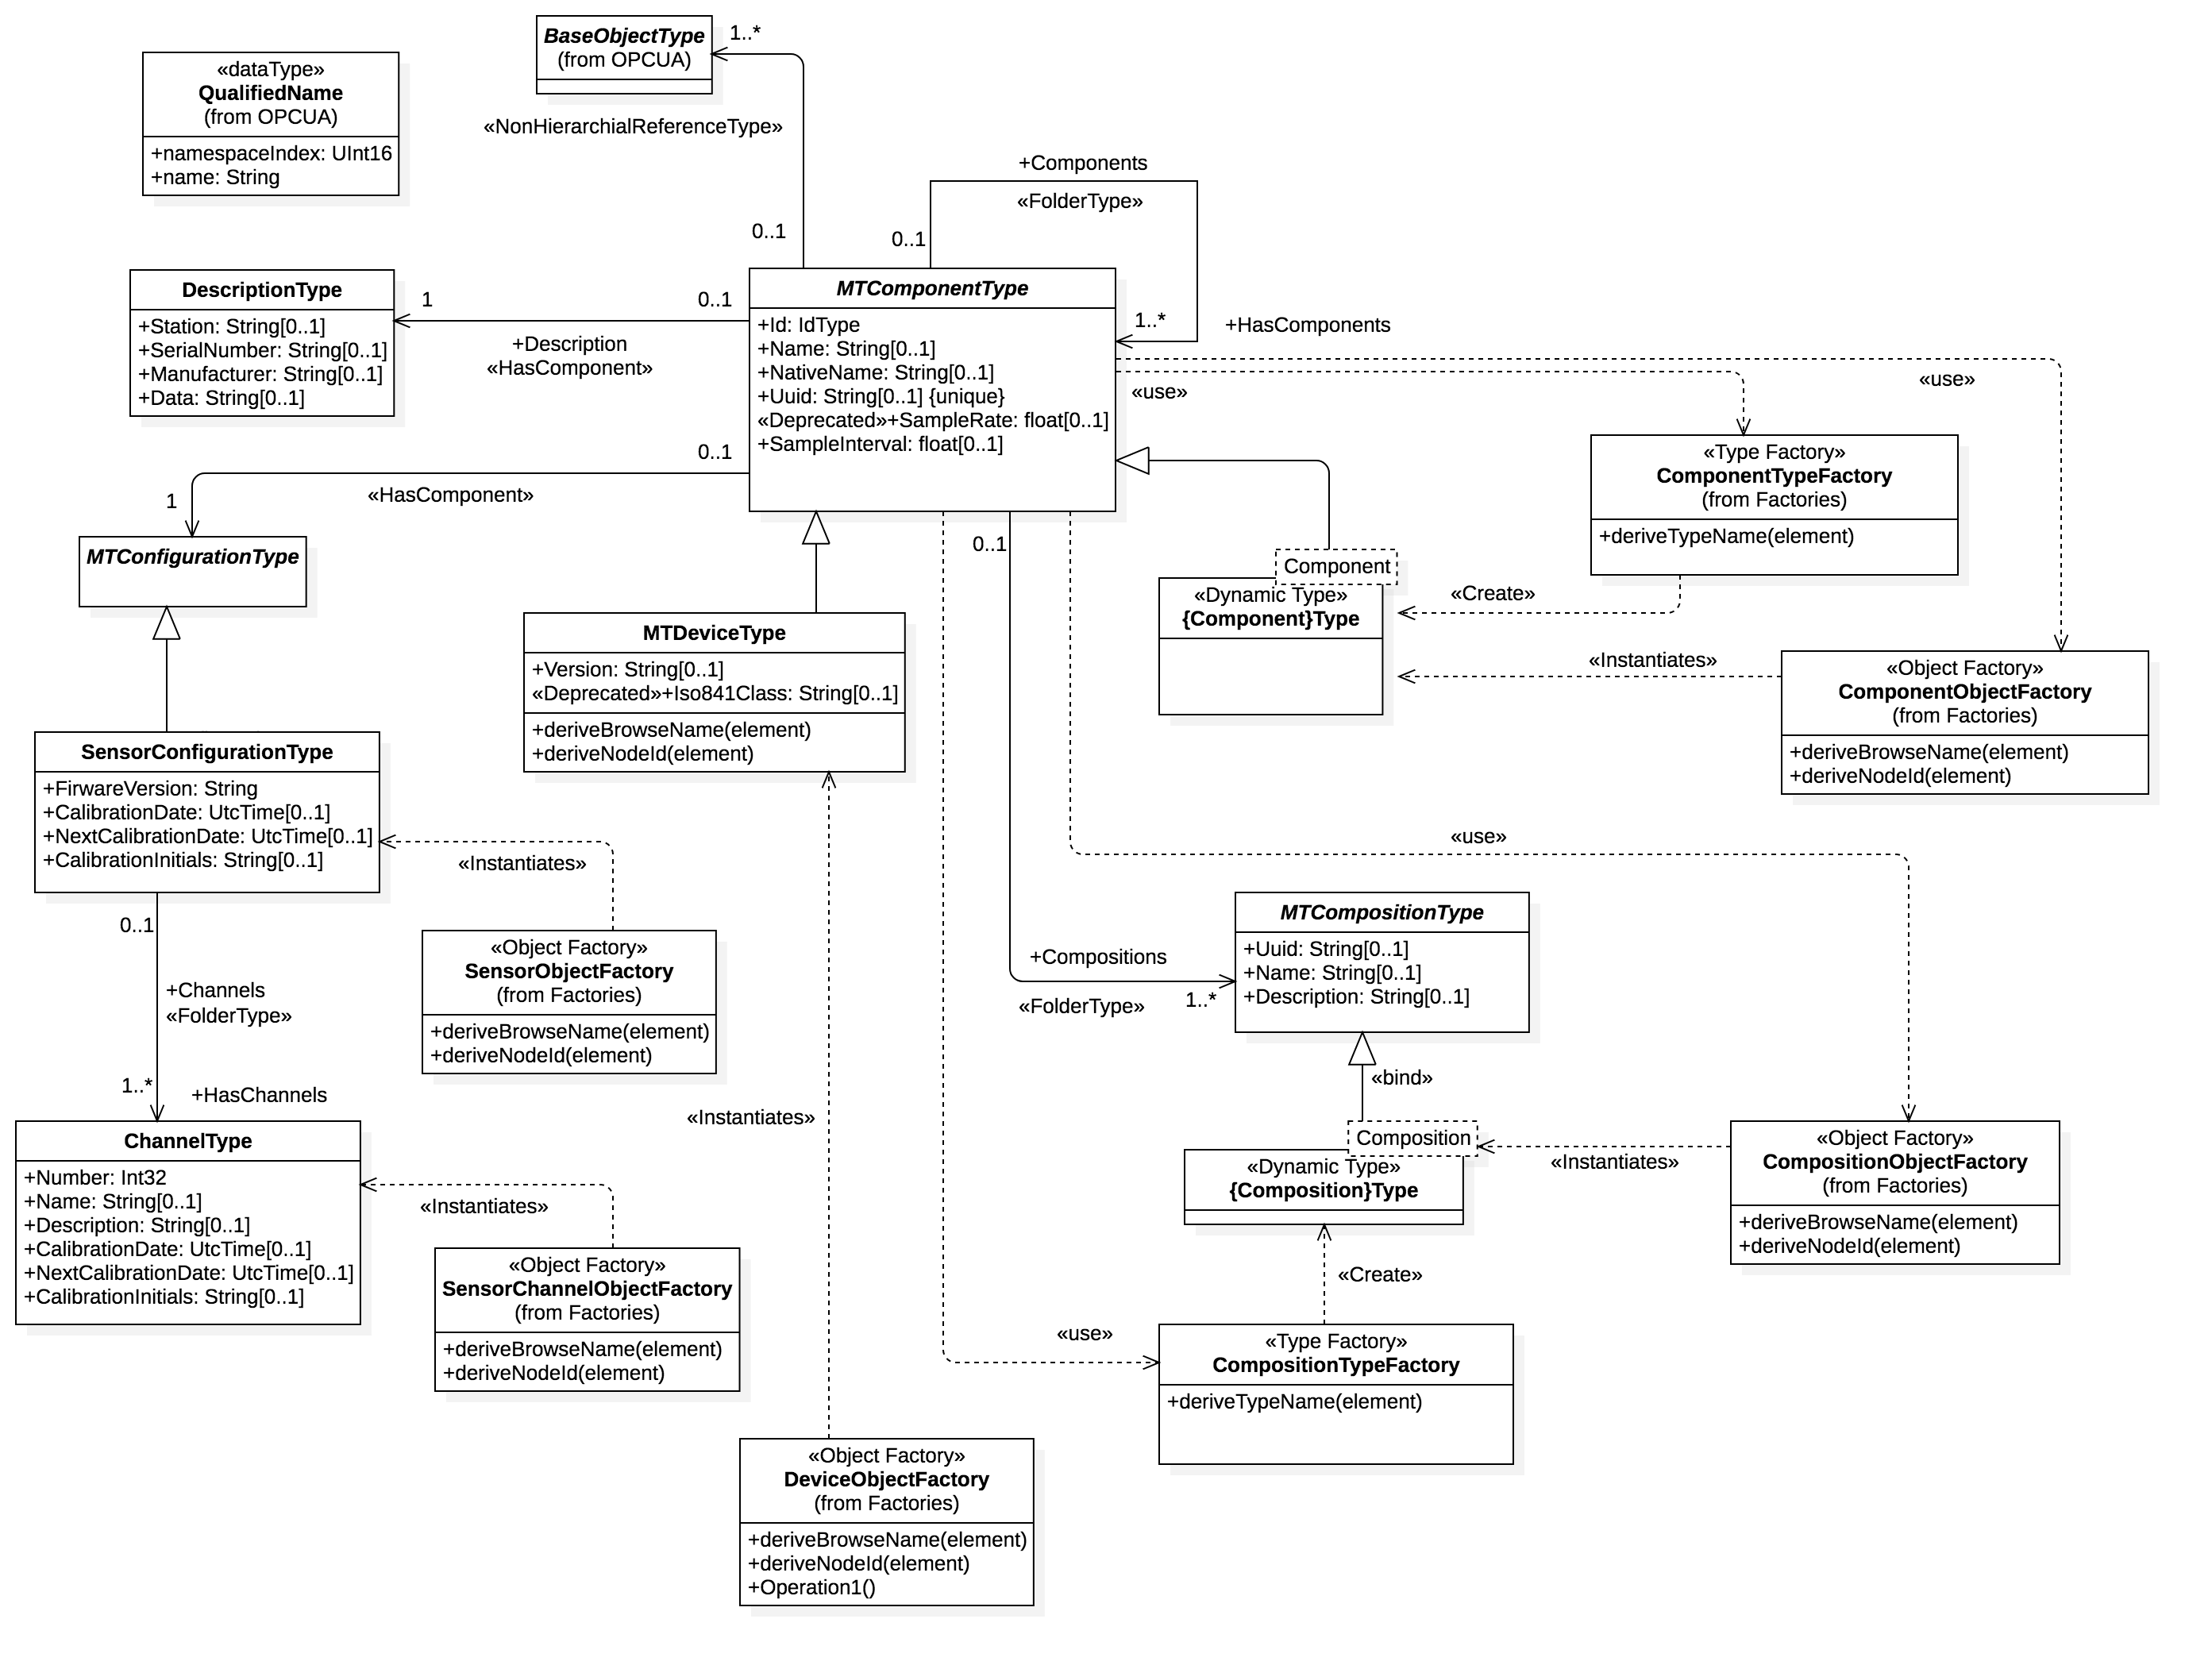
\includegraphics[width=1.0\textwidth]{diagrams/Components.png}
  \caption{Components Diagram}
  \label{fig:Components}
\end{figure}

\FloatBarrier


The Components documents the Component models and the owned objects.

\subsubsection{Defintion of \texttt{ ChannelType}} \label{type:ChannelType}

\FloatBarrier

An MTConnect \texttt{Channel} is a single data stream associated with a sensor. Each stream
of data can be calibrated separately and allows for the specification of the meta information
and descriptive information. The only required property of the \texttt{Channel} is the number
which is the unique identifier.

The channels will be created by the \texttt{SensorChannelObjectFactory} that composes the \texttt{BrowseName} 
and the \texttt{NodeId} for each object. (See \ref{type:SensorChannelObjectFactory}).

\begin{table}[ht]
\centering 
  \caption{\texttt{ChannelType} Definition}
  \label{table:ChannelType}
\fontsize{9pt}{11pt}\selectfont
\tabulinesep=3pt
\begin{tabu} to 6in {|l|l|l|l|l|l|} \everyrow{\hline}
\hline
\rowfont\bfseries {Attribute} & \multicolumn{5}{|l|}{Value} \\
\tabucline[1.5pt]{}
BrowseName & \multicolumn{5}{|l|}{ChannelType} \\
IsAbstract & \multicolumn{5}{|l|}{False} \\
\tabucline[1.5pt]{}
\rowfont \bfseries References & NodeClass & BrowseName & DataType & TypeDefinition & {Modeling Rule} \\
\multicolumn{6}{|l|}{Subtype of BaseObjectType (See OPCUA Documentation)} \\
HasProperty & Variable & Number &  Int32 & PropertyType & Mandatory \\
HasProperty & Variable & Name &  String & PropertyType & Optional \\
HasProperty & Variable & MTDescription &  String & PropertyType & Optional \\
HasProperty & Variable & CalibrationDate &  UtcTime & PropertyType & Optional \\
HasProperty & Variable & NextCalibrationDate &  UtcTime & PropertyType & Optional \\
HasProperty & Variable & CalibrationInitials &  String & PropertyType & Optional \\
\end{tabu}
\end{table} 


\FloatBarrier
\subsubsection{Defintion of \texttt{ DescriptionType}} \label{type:DescriptionType}

\FloatBarrier

The desription provides some general information about the 
manufacture and serial number of the component. In the XML, the \texttt{CDATA} is freeform 
text that is represented in the \texttt{Data} Property of the Description Object. The description is 
related to the component with the OPC/UA \texttt{HasComponent} relationship.

\begin{table}[ht]
\centering 
  \caption{\texttt{DescriptionType} Definition}
  \label{table:DescriptionType}
\fontsize{9pt}{11pt}\selectfont
\tabulinesep=3pt
\begin{tabu} to 6in {|l|l|l|l|l|l|} \everyrow{\hline}
\hline
\rowfont\bfseries {Attribute} & \multicolumn{5}{|l|}{Value} \\
\tabucline[1.5pt]{}
BrowseName & \multicolumn{5}{|l|}{DescriptionType} \\
IsAbstract & \multicolumn{5}{|l|}{False} \\
\tabucline[1.5pt]{}
\rowfont \bfseries References & NodeClass & BrowseName & DataType & TypeDefinition & {Modeling Rule} \\
\multicolumn{6}{|l|}{Subtype of BaseObjectType (See OPCUA Documentation)} \\
HasProperty & Variable & Station &  String & PropertyType & Optional \\
HasProperty & Variable & SerialNumber &  String & PropertyType & Optional \\
HasProperty & Variable & Manufacturer &  String & PropertyType & Optional \\
HasProperty & Variable & Data &  String & PropertyType & Optional \\
\end{tabu}
\end{table} 


\paragraph{Operations}
\begin{itemize}
  \item \texttt{deriveBrowseName(element)}\\
    Specification:
   \indent \begin{Verbatim}[xleftmargin=.25in,fontsize=\small]
"Description"
\end{Verbatim}

  \item \texttt{deriveNodeId(element)}\\
    Specification:
   \indent \begin{Verbatim}[xleftmargin=.25in,fontsize=\small]
concat(self.parent.NodeId, BrowseName)
\end{Verbatim}

\end{itemize}
\FloatBarrier
\subsubsection{Defintion of \texttt{ MTComponentType}} \label{type:MTComponentType}

\FloatBarrier

The base Component Type from which all MTConnect Components are derived. The 
component type factory is used to create the specific OPC/UA Types as subtypes of the 
MTConnect \texttt{MTComponentType}. The component types will be created once for all Component objects 
of that type based on the \texttt{QName} of the MTConnect XML element. 

The object factory will instantiate the Component Objects and insert them into the Components 
folder with a browse name of the Component QName and the \texttt{name} element if specified surrounded 
by square brackets, \texttt{[]}. For example if the MTConnect Element is:

\texttt{<Linear name='X'>...</...>}

The OPC/UA Object with browse name \texttt{Linear[X]} will be created with the HasTypeDefinition 
referencing the \texttt{Linear} OPC/UA type. 

The meta data for the component and it's relationships are static. The dynamic data will be 
represented using the \textit{OPC/UA Part 8}.



\begin{table}[ht]
\centering 
  \caption{\texttt{MTComponentType} Definition}
  \label{table:MTComponentType}
\fontsize{9pt}{11pt}\selectfont
\tabulinesep=3pt
\begin{tabu} to 6in {|l|l|l|l|l|l|} \everyrow{\hline}
\hline
\rowfont\bfseries {Attribute} & \multicolumn{5}{|l|}{Value} \\
\tabucline[1.5pt]{}
BrowseName & \multicolumn{5}{|l|}{MTComponentType} \\
IsAbstract & \multicolumn{5}{|l|}{True} \\
\tabucline[1.5pt]{}
\rowfont \bfseries References & NodeClass & BrowseName & DataType & TypeDefinition & {Modeling Rule} \\
HasSubtype & ObjectType & MTDeviceType & \multicolumn{3}{|l|}{See section \ref{type:MTDeviceType}} \\
HasSubtype & ObjectType & \{Component\}Type & \multicolumn{3}{|l|}{See section \ref{type:{Component}Type}} \\
HasProperty & Variable & XmlId &  IdType & PropertyType & Mandatory \\
HasProperty & Variable & Name &  String & PropertyType & Optional \\
HasProperty & Variable & NativeName &  String & PropertyType & Optional \\
HasProperty & Variable & Uuid &  String & PropertyType & Optional \\
HasProperty & Variable & SampleRate &  float & PropertyType & Optional \\
HasProperty & Variable & SampleInterval &  float & PropertyType & Optional \\
HasComponent & Object & Description &   & DescriptionType & Optional \\
HasComponent & Object & Configuration &   & MTConfigurationType & Optional \\
Organizes & Object & Components &  MTComponentType & FolderType & Optional \\
Organizes & Object & Compositions &  MTCompositionType & FolderType & Optional \\
HasProperty & Variable & <Dynamic> &  BaseObjectType & <Dynamic> & Optional \\
Organizes & Object & Conditions &  AlarmConditionType & FolderType & Optional \\
HasProperty & Variable & <Dynamic> &  {DataItem}Type & <Dynamic> & Optional \\
\end{tabu}
\end{table} 


\paragraph{Constraints}
\begin{itemize}
\item Constraint \texttt{node_id}: 
   \indent \begin{Verbatim}[xleftmargin=.25in,fontsize=\small]
context Component::NodeId : String 
derive: concat(self.getDevice().uuid, self.getAttributes().id)
\end{Verbatim}
Documentation: The NodeId SHALL be derrived from the combination of the device UUID and the id of the component. 

\end{itemize}
\paragraph{Dependency on DataItemTypeFactory}

This class relates to \texttt{DataItemTypeFactory} (See section \ref{type:DataItemTypeFactory}) for a(n) \texttt{use} relationship.

\paragraph{Dependency on DataItemObjectFactory}

This class relates to \texttt{DataItemObjectFactory} (See section \ref{type:DataItemObjectFactory}) for a(n) \texttt{use} relationship.

\paragraph{Dependency on CompositionObjectFactory}

This class relates to \texttt{CompositionObjectFactory} (See section \ref{type:CompositionObjectFactory}) for a(n) \texttt{use} relationship.

\paragraph{Dependency on CompositionTypeFactory}

This class relates to \texttt{CompositionTypeFactory} (See section \ref{type:CompositionTypeFactory}) for a(n) \texttt{use} relationship.

\FloatBarrier
\subsubsection{Defintion of \texttt{ MTCompositionType}} \label{type:MTCompositionType}

\FloatBarrier

The \texttt{MTCompositionType} is the abstract supertype of the dynamically generated
composition types based on the attribute \texttt{type} of the \texttt{Composition} element
of the MTConnect \texttt{Component}. The \texttt{Composition} is then related to the 
DataItems that reference the \texttt{Composition}'s id in their \texttt{compositionId} 
attribute. 

The data items are added to the relationship where the \texttt{DataItem} to \texttt{Composition} 
relationship is represented by the \texttt{BrowseName} Composition property of the data item 
the data items are added by their browse names to the \texttt{Composition}.

\begin{table}[ht]
\centering 
  \caption{\texttt{MTCompositionType} Definition}
  \label{table:MTCompositionType}
\fontsize{9pt}{11pt}\selectfont
\tabulinesep=3pt
\begin{tabu} to 6in {|l|l|l|l|l|l|} \everyrow{\hline}
\hline
\rowfont\bfseries {Attribute} & \multicolumn{5}{|l|}{Value} \\
\tabucline[1.5pt]{}
BrowseName & \multicolumn{5}{|l|}{MTCompositionType} \\
IsAbstract & \multicolumn{5}{|l|}{True} \\
\tabucline[1.5pt]{}
\rowfont \bfseries References & NodeClass & BrowseName & DataType & TypeDefinition & {Modeling Rule} \\
\multicolumn{6}{|l|}{Subtype of BaseObjectType (See OPCUA Documentation)} \\
HasSubtype & ObjectType & \{Composition\}Type & \multicolumn{3}{|l|}{See section \ref{type:{Composition}Type}} \\
HasProperty & Variable & Uuid &  String & PropertyType & Optional \\
HasProperty & Variable & Name &  String & PropertyType & Optional \\
HasProperty & Variable & MTDescription &  String & PropertyType & Optional \\
NonHierarchialReferenceType & Object & <DataItem> &  {DataItem}Type & NonHierarchialReferenceType & Optional \\
\end{tabu}
\end{table} 


\FloatBarrier
\subsubsection{Defintion of \texttt{ MTConfigurationType}} \label{type:MTConfigurationType}

\FloatBarrier

The abstract \texttt{MTConfigurationType} currently has only one sub-type, \\
\texttt{SensorConfigurationType} (see 
\ref{type:SensorConfigurationType}). In the future the configurations will also contain component 
and device configuration information as sub-types. 

\begin{table}[ht]
\centering 
  \caption{\texttt{MTConfigurationType} Definition}
  \label{table:MTConfigurationType}
\fontsize{9pt}{11pt}\selectfont
\tabulinesep=3pt
\begin{tabu} to 6in {|l|l|l|l|l|l|} \everyrow{\hline}
\hline
\rowfont\bfseries {Attribute} & \multicolumn{5}{|l|}{Value} \\
\tabucline[1.5pt]{}
BrowseName & \multicolumn{5}{|l|}{MTConfigurationType} \\
IsAbstract & \multicolumn{5}{|l|}{True} \\
\tabucline[1.5pt]{}
\rowfont \bfseries References & NodeClass & BrowseName & DataType & TypeDefinition & {Modeling Rule} \\
\multicolumn{6}{|l|}{Subtype of BaseObjectType (See OPCUA Documentation)} \\
HasSubtype & ObjectType & SensorConfigurationType & \multicolumn{3}{|l|}{See section \ref{type:SensorConfigurationType}} \\
\end{tabu}
\end{table} 


\FloatBarrier
\subsubsection{Defintion of \texttt{ MTDeviceType}} \label{type:MTDeviceType}

\FloatBarrier

The MTDevice is a special type whose object will be the root of the device graph. The Device uses the component type factory and the component object factories to create each of the first level components. 

The  compositions, relationships, and data items are then recursively created as one decendes the MTConnect informaiton model.

\begin{table}[ht]
\centering 
  \caption{\texttt{MTDeviceType} Definition}
  \label{table:MTDeviceType}
\fontsize{9pt}{11pt}\selectfont
\tabulinesep=3pt
\begin{tabu} to 6in {|l|l|l|l|l|l|} \everyrow{\hline}
\hline
\rowfont\bfseries {Attribute} & \multicolumn{5}{|l|}{Value} \\
\tabucline[1.5pt]{}
BrowseName & \multicolumn{5}{|l|}{MTDeviceType} \\
IsAbstract & \multicolumn{5}{|l|}{False} \\
\tabucline[1.5pt]{}
\rowfont \bfseries References & NodeClass & BrowseName & DataType & TypeDefinition & {Modeling Rule} \\
\multicolumn{6}{|l|}{Subtype of MTComponentType (See section \ref{type:MTComponentType})} \\
HasProperty & Variable & Version &  String & PropertyType & Optional \\
HasProperty & Variable & Iso841Class &  String & PropertyType & Optional \\
\end{tabu}
\end{table} 


\paragraph{Operations}
\begin{itemize}
  \item \texttt{deriveBrowseName(element)}\\
    Specification:
   \indent \begin{Verbatim}[xleftmargin=.25in,fontsize=\small]
self.name
\end{Verbatim}

  \item \texttt{deriveNodeId(element)}\\
    Specification:
   \indent \begin{Verbatim}[xleftmargin=.25in,fontsize=\small]
self.uuid
\end{Verbatim}

\end{itemize}
\paragraph{Constraints}
\begin{itemize}
\item Constraint \texttt{uuid_not_empty}: 
   \indent \begin{Verbatim}[xleftmargin=.25in,fontsize=\small]
uuid->notEmpty()
\end{Verbatim}
Documentation: The  UUID SHALL be provided.

\end{itemize}
\begin{itemize}
\item Constraint \texttt{name_not_empty}: 
   \indent \begin{Verbatim}[xleftmargin=.25in,fontsize=\small]
name->notEmpty()
\end{Verbatim}
Documentation: The name of the Device SHALL be given.

\end{itemize}
\paragraph{Dependency on ComponentTypeFactory}

This class relates to \texttt{ComponentTypeFactory} (See section \ref{type:ComponentTypeFactory}) for a(n) \texttt{use} relationship.

\paragraph{Dependency on ComponentObjectFactory}

This class relates to \texttt{ComponentObjectFactory} (See section \ref{type:ComponentObjectFactory}) for a(n) \texttt{use} relationship.

\FloatBarrier
\subsubsection{Defintion of \texttt{ SensorConfigurationType}} \label{type:SensorConfigurationType}

\FloatBarrier

The SensorConfiguration browse name will be created as an Object relationship with the parent component.

\begin{table}[ht]
\centering 
  \caption{\texttt{SensorConfigurationType} Definition}
  \label{table:SensorConfigurationType}
\fontsize{9pt}{11pt}\selectfont
\tabulinesep=3pt
\begin{tabu} to 6in {|l|l|l|l|l|l|} \everyrow{\hline}
\hline
\rowfont\bfseries {Attribute} & \multicolumn{5}{|l|}{Value} \\
\tabucline[1.5pt]{}
BrowseName & \multicolumn{5}{|l|}{SensorConfigurationType} \\
IsAbstract & \multicolumn{5}{|l|}{False} \\
\tabucline[1.5pt]{}
\rowfont \bfseries References & NodeClass & BrowseName & DataType & TypeDefinition & {Modeling Rule} \\
\multicolumn{6}{|l|}{Subtype of MTConfigurationType (See section \ref{type:MTConfigurationType})} \\
HasProperty & Variable & FirwareVersion &  String & PropertyType & Mandatory \\
HasProperty & Variable & CalibrationDate &  UtcTime & PropertyType & Optional \\
HasProperty & Variable & NextCalibrationDate &  UtcTime & PropertyType & Optional \\
HasProperty & Variable & CalibrationInitials &  String & PropertyType & Optional \\
Organizes & Object & Channels &  ChannelType & FolderType & Optional \\
\end{tabu}
\end{table} 


\FloatBarrier
\subsubsection{Defintion of \texttt{<<Dynamic Type>> \{Component\}Type}} \label{type:{Component}Type}

\FloatBarrier



\begin{table}[ht]
\centering 
  \caption{\texttt{\{Component\}Type} Definition}
  \label{table:{Component}Type}
\fontsize{9pt}{11pt}\selectfont
\tabulinesep=3pt
\begin{tabu} to 6in {|l|l|l|l|l|l|} \everyrow{\hline}
\hline
\rowfont\bfseries {Attribute} & \multicolumn{5}{|l|}{Value} \\
\tabucline[1.5pt]{}
BrowseName & \multicolumn{5}{|l|}{{Component}Type} \\
IsAbstract & \multicolumn{5}{|l|}{False} \\
\tabucline[1.5pt]{}
\rowfont \bfseries References & NodeClass & BrowseName & DataType & TypeDefinition & {Modeling Rule} \\
\multicolumn{6}{|l|}{Subtype of MTComponentType (See section \ref{type:MTComponentType})} \\
\end{tabu}
\end{table} 


\FloatBarrier
\subsubsection{Defintion of \texttt{<<Dynamic Type>> \{Composition\}Type}} \label{type:{Composition}Type}

\FloatBarrier



\begin{table}[ht]
\centering 
  \caption{\texttt{\{Composition\}Type} Definition}
  \label{table:{Composition}Type}
\fontsize{9pt}{11pt}\selectfont
\tabulinesep=3pt
\begin{tabu} to 6in {|l|l|l|l|l|l|} \everyrow{\hline}
\hline
\rowfont\bfseries {Attribute} & \multicolumn{5}{|l|}{Value} \\
\tabucline[1.5pt]{}
BrowseName & \multicolumn{5}{|l|}{{Composition}Type} \\
IsAbstract & \multicolumn{5}{|l|}{False} \\
\tabucline[1.5pt]{}
\rowfont \bfseries References & NodeClass & BrowseName & DataType & TypeDefinition & {Modeling Rule} \\
\multicolumn{6}{|l|}{Subtype of MTCompositionType (See section \ref{type:MTCompositionType})} \\
\end{tabu}
\end{table} 


\FloatBarrier
\subsection{Data Items}

\begin{figure}[ht]
  \centering
    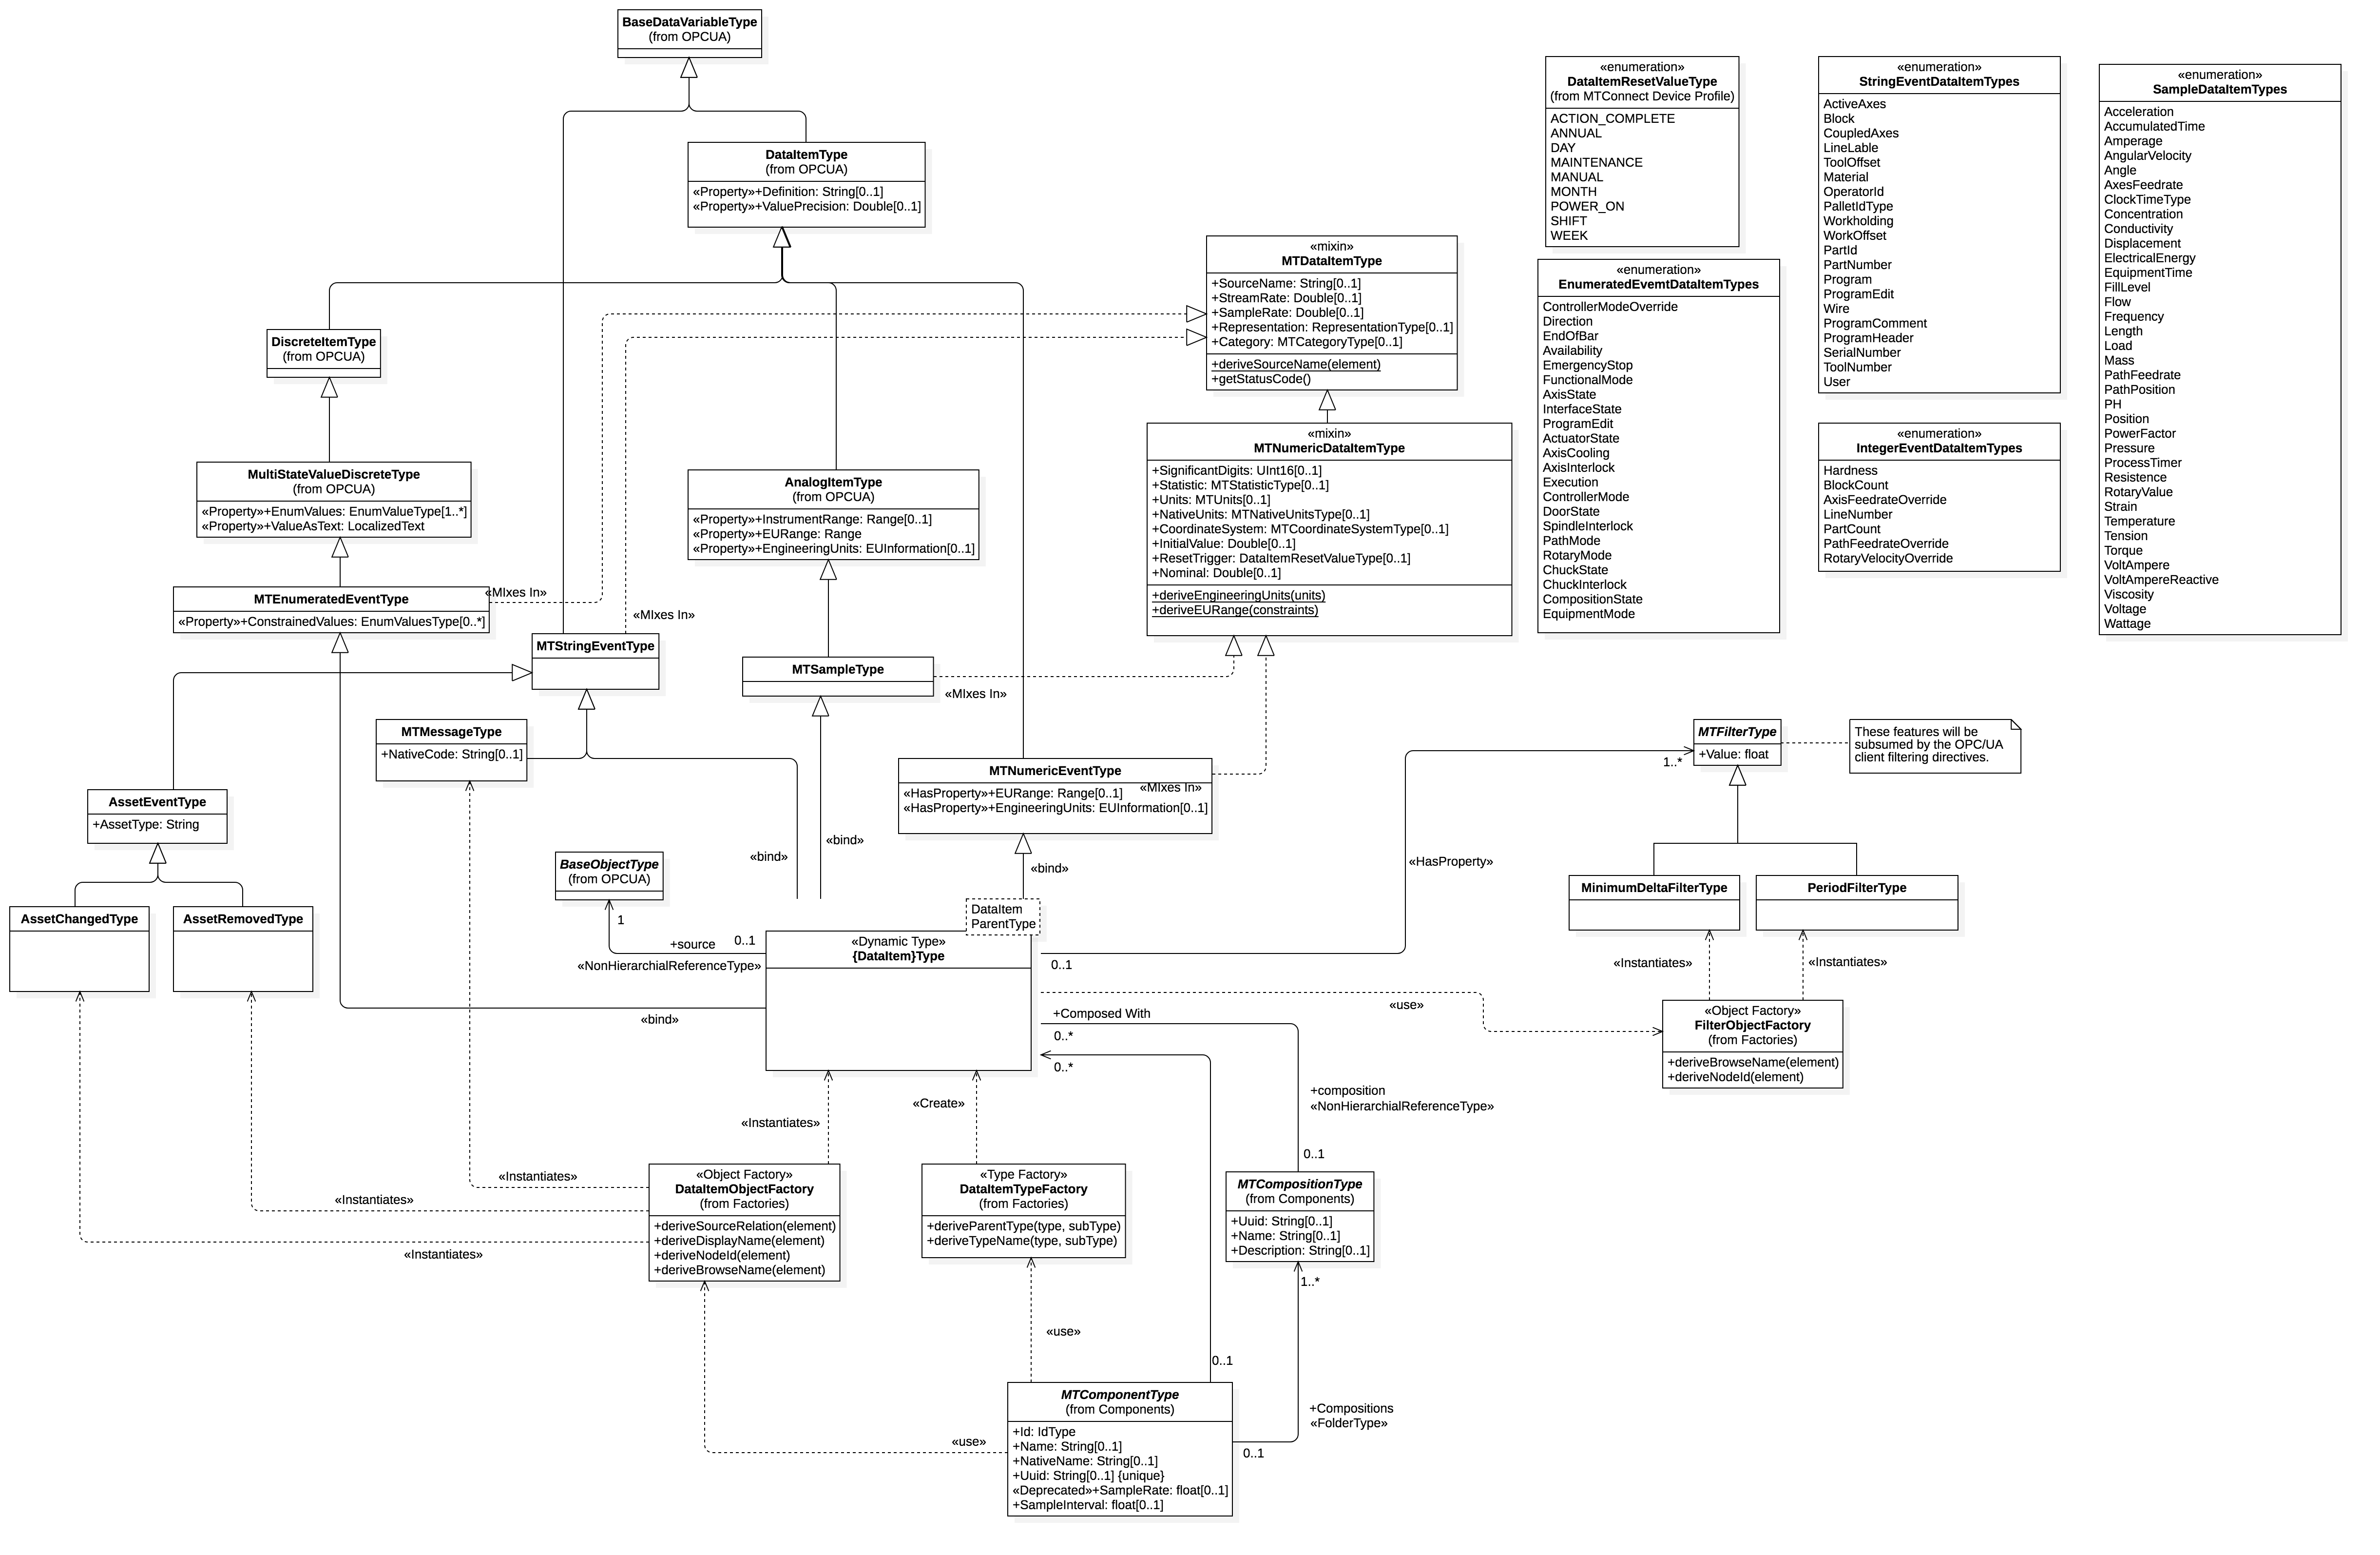
\includegraphics[width=1.0\textwidth]{diagrams/Data Items.png}
  \caption{Data Items Diagram}
  \label{fig:Data Items}
\end{figure}

\FloatBarrier




\subsubsection{Defintion of \texttt{ ActuatorStateType}} \label{type:ActuatorStateType}

\FloatBarrier

See \texttt{ActuatorState} in section 6.2 Event \textit{Element Names}
of MTConnect Part 3 -- Streams Information Model.

\begin{table}[ht]
\centering 
  \caption{\texttt{ActuatorStateType} Definition}
  \label{table:ActuatorStateType}
\fontsize{9pt}{11pt}\selectfont
\tabulinesep=3pt
\begin{tabu} to 6in {|l|l|l|l|l|l|} \everyrow{\hline}
\hline
\rowfont\bfseries {Attribute} & \multicolumn{5}{|l|}{Value} \\
\tabucline[1.5pt]{}
BrowseName & \multicolumn{5}{|l|}{ActuatorStateType} \\
IsAbstract & \multicolumn{5}{|l|}{False} \\
ValueRank & \multicolumn{5}{|l|}{-1} \\
DataType & \multicolumn{5}{|l|}{Number} \\
\tabucline[1.5pt]{}
\rowfont \bfseries References & NodeClass & BrowseName & DataType & TypeDefinition & {Modeling Rule} \\
\multicolumn{6}{|l|}{Subtype of MTEnumeratedEventType (See section \ref{type:MTEnumeratedEventType})} \\
\end{tabu}
\end{table} 


\paragraph{Allowable Values}
\begin{table}[ht]
\centering 
  \caption{\texttt{ActiveStateValues} Enumeration}
\tabulinesep=3pt
\begin{tabu} to 6in {|l|r|} \everyrow{\hline}
\hline
\rowfont\bfseries {Name} & {Index} \\
\tabucline[1.5pt]{}
\texttt{ACTIVE} & \texttt{0} \\
\texttt{INACTIVE} & \texttt{1} \\
\end{tabu}
\end{table} 
\FloatBarrier
\subsubsection{Defintion of \texttt{ AssetChangedType}} \label{type:AssetChangedType}

\FloatBarrier



\begin{table}[ht]
\centering 
  \caption{\texttt{AssetChangedType} Definition}
  \label{table:AssetChangedType}
\fontsize{9pt}{11pt}\selectfont
\tabulinesep=3pt
\begin{tabu} to 6in {|l|l|l|l|l|l|} \everyrow{\hline}
\hline
\rowfont\bfseries {Attribute} & \multicolumn{5}{|l|}{Value} \\
\tabucline[1.5pt]{}
BrowseName & \multicolumn{5}{|l|}{AssetChangedType} \\
IsAbstract & \multicolumn{5}{|l|}{False} \\
ValueRank & \multicolumn{5}{|l|}{-1} \\
DataType & \multicolumn{5}{|l|}{String} \\
\tabucline[1.5pt]{}
\rowfont \bfseries References & NodeClass & BrowseName & DataType & TypeDefinition & {Modeling Rule} \\
\multicolumn{6}{|l|}{Subtype of AssetEventType (See section \ref{type:AssetEventType})} \\
\end{tabu}
\end{table} 


\FloatBarrier
\subsubsection{Defintion of \texttt{ AssetEventType}} \label{type:AssetEventType}

\FloatBarrier



\begin{table}[ht]
\centering 
  \caption{\texttt{AssetEventType} Definition}
  \label{table:AssetEventType}
\fontsize{9pt}{11pt}\selectfont
\tabulinesep=3pt
\begin{tabu} to 6in {|l|l|l|l|l|l|} \everyrow{\hline}
\hline
\rowfont\bfseries {Attribute} & \multicolumn{5}{|l|}{Value} \\
\tabucline[1.5pt]{}
BrowseName & \multicolumn{5}{|l|}{AssetEventType} \\
IsAbstract & \multicolumn{5}{|l|}{False} \\
ValueRank & \multicolumn{5}{|l|}{-1} \\
DataType & \multicolumn{5}{|l|}{String} \\
\tabucline[1.5pt]{}
\rowfont \bfseries References & NodeClass & BrowseName & DataType & TypeDefinition & {Modeling Rule} \\
\multicolumn{6}{|l|}{Subtype of MTStringEventType (See section \ref{type:MTStringEventType})} \\
HasSubtype & VariableType & AssetChangedType & \multicolumn{3}{|l|}{See section \ref{type:AssetChangedType}} \\
HasSubtype & VariableType & AssetRemovedType & \multicolumn{3}{|l|}{See section \ref{type:AssetRemovedType}} \\
HasProperty & Variable & AssetType &  String & PropertyType & Mandatory \\
\end{tabu}
\end{table} 


\FloatBarrier
\subsubsection{Defintion of \texttt{ AssetRemovedType}} \label{type:AssetRemovedType}

\FloatBarrier



\begin{table}[ht]
\centering 
  \caption{\texttt{AssetRemovedType} Definition}
  \label{table:AssetRemovedType}
\fontsize{9pt}{11pt}\selectfont
\tabulinesep=3pt
\begin{tabu} to 6in {|l|l|l|l|l|l|} \everyrow{\hline}
\hline
\rowfont\bfseries {Attribute} & \multicolumn{5}{|l|}{Value} \\
\tabucline[1.5pt]{}
BrowseName & \multicolumn{5}{|l|}{AssetRemovedType} \\
IsAbstract & \multicolumn{5}{|l|}{False} \\
ValueRank & \multicolumn{5}{|l|}{-1} \\
DataType & \multicolumn{5}{|l|}{String} \\
\tabucline[1.5pt]{}
\rowfont \bfseries References & NodeClass & BrowseName & DataType & TypeDefinition & {Modeling Rule} \\
\multicolumn{6}{|l|}{Subtype of AssetEventType (See section \ref{type:AssetEventType})} \\
\end{tabu}
\end{table} 


\FloatBarrier
\subsubsection{Defintion of \texttt{ AvailabilityType}} \label{type:AvailabilityType}

\FloatBarrier



\begin{table}[ht]
\centering 
  \caption{\texttt{AvailabilityType} Definition}
  \label{table:AvailabilityType}
\fontsize{9pt}{11pt}\selectfont
\tabulinesep=3pt
\begin{tabu} to 6in {|l|l|l|l|l|l|} \everyrow{\hline}
\hline
\rowfont\bfseries {Attribute} & \multicolumn{5}{|l|}{Value} \\
\tabucline[1.5pt]{}
BrowseName & \multicolumn{5}{|l|}{AvailabilityType} \\
IsAbstract & \multicolumn{5}{|l|}{False} \\
ValueRank & \multicolumn{5}{|l|}{-1} \\
DataType & \multicolumn{5}{|l|}{Number} \\
\tabucline[1.5pt]{}
\rowfont \bfseries References & NodeClass & BrowseName & DataType & TypeDefinition & {Modeling Rule} \\
\multicolumn{6}{|l|}{Subtype of MTEnumeratedEventType (See section \ref{type:MTEnumeratedEventType})} \\
\end{tabu}
\end{table} 


\paragraph{Allowable Values}
\begin{table}[ht]
\centering 
  \caption{\texttt{AvailabilityValues} Enumeration}
\tabulinesep=3pt
\begin{tabu} to 6in {|l|r|} \everyrow{\hline}
\hline
\rowfont\bfseries {Name} & {Index} \\
\tabucline[1.5pt]{}
\texttt{AVAILABILE} & \texttt{0} \\
\texttt{UNAVAILABLE} & \texttt{1} \\
\end{tabu}
\end{table} 
\FloatBarrier
\subsubsection{Defintion of \texttt{ AxisCouplingType}} \label{type:AxisCouplingType}

\FloatBarrier



\begin{table}[ht]
\centering 
  \caption{\texttt{AxisCouplingType} Definition}
  \label{table:AxisCouplingType}
\fontsize{9pt}{11pt}\selectfont
\tabulinesep=3pt
\begin{tabu} to 6in {|l|l|l|l|l|l|} \everyrow{\hline}
\hline
\rowfont\bfseries {Attribute} & \multicolumn{5}{|l|}{Value} \\
\tabucline[1.5pt]{}
BrowseName & \multicolumn{5}{|l|}{AxisCouplingType} \\
IsAbstract & \multicolumn{5}{|l|}{False} \\
ValueRank & \multicolumn{5}{|l|}{-1} \\
DataType & \multicolumn{5}{|l|}{Number} \\
\tabucline[1.5pt]{}
\rowfont \bfseries References & NodeClass & BrowseName & DataType & TypeDefinition & {Modeling Rule} \\
\multicolumn{6}{|l|}{Subtype of MTEnumeratedEventType (See section \ref{type:MTEnumeratedEventType})} \\
\end{tabu}
\end{table} 


\paragraph{Allowable Values}
\begin{table}[ht]
\centering 
  \caption{\texttt{AxisCouplingValues} Enumeration}
\tabulinesep=3pt
\begin{tabu} to 6in {|l|r|} \everyrow{\hline}
\hline
\rowfont\bfseries {Name} & {Index} \\
\tabucline[1.5pt]{}
\texttt{MASTER} & \texttt{0} \\
\texttt{SLAVE} & \texttt{1} \\
\texttt{SYNCHRONOUS} & \texttt{2} \\
\texttt{TANDEM} & \texttt{3} \\
\end{tabu}
\end{table} 
\FloatBarrier
\subsubsection{Defintion of \texttt{ AxisInterlockType}} \label{type:AxisInterlockType}

\FloatBarrier



\begin{table}[ht]
\centering 
  \caption{\texttt{AxisInterlockType} Definition}
  \label{table:AxisInterlockType}
\fontsize{9pt}{11pt}\selectfont
\tabulinesep=3pt
\begin{tabu} to 6in {|l|l|l|l|l|l|} \everyrow{\hline}
\hline
\rowfont\bfseries {Attribute} & \multicolumn{5}{|l|}{Value} \\
\tabucline[1.5pt]{}
BrowseName & \multicolumn{5}{|l|}{AxisInterlockType} \\
IsAbstract & \multicolumn{5}{|l|}{False} \\
ValueRank & \multicolumn{5}{|l|}{-1} \\
DataType & \multicolumn{5}{|l|}{Number} \\
\tabucline[1.5pt]{}
\rowfont \bfseries References & NodeClass & BrowseName & DataType & TypeDefinition & {Modeling Rule} \\
\multicolumn{6}{|l|}{Subtype of MTEnumeratedEventType (See section \ref{type:MTEnumeratedEventType})} \\
\end{tabu}
\end{table} 


\paragraph{Allowable Values}
\begin{table}[ht]
\centering 
  \caption{\texttt{ActiveStateValues} Enumeration}
\tabulinesep=3pt
\begin{tabu} to 6in {|l|r|} \everyrow{\hline}
\hline
\rowfont\bfseries {Name} & {Index} \\
\tabucline[1.5pt]{}
\texttt{ACTIVE} & \texttt{0} \\
\texttt{INACTIVE} & \texttt{1} \\
\end{tabu}
\end{table} 
\FloatBarrier
\subsubsection{Defintion of \texttt{ AxisStateType}} \label{type:AxisStateType}

\FloatBarrier



\begin{table}[ht]
\centering 
  \caption{\texttt{AxisStateType} Definition}
  \label{table:AxisStateType}
\fontsize{9pt}{11pt}\selectfont
\tabulinesep=3pt
\begin{tabu} to 6in {|l|l|l|l|l|l|} \everyrow{\hline}
\hline
\rowfont\bfseries {Attribute} & \multicolumn{5}{|l|}{Value} \\
\tabucline[1.5pt]{}
BrowseName & \multicolumn{5}{|l|}{AxisStateType} \\
IsAbstract & \multicolumn{5}{|l|}{False} \\
\tabucline[1.5pt]{}
\rowfont \bfseries References & NodeClass & BrowseName & DataType & TypeDefinition & {Modeling Rule} \\
\end{tabu}
\end{table} 


\paragraph{Allowable Values}
\begin{table}[ht]
\centering 
  \caption{\texttt{AxisStateValues} Enumeration}
\tabulinesep=3pt
\begin{tabu} to 6in {|l|r|} \everyrow{\hline}
\hline
\rowfont\bfseries {Name} & {Index} \\
\tabucline[1.5pt]{}
\texttt{HOME} & \texttt{0} \\
\texttt{PARKED} & \texttt{1} \\
\texttt{STOPPED} & \texttt{2} \\
\texttt{TRAVEL} & \texttt{3} \\
\end{tabu}
\end{table} 
\FloatBarrier
\subsubsection{Defintion of \texttt{ ChuckInterlockType}} \label{type:ChuckInterlockType}

\FloatBarrier



\begin{table}[ht]
\centering 
  \caption{\texttt{ChuckInterlockType} Definition}
  \label{table:ChuckInterlockType}
\fontsize{9pt}{11pt}\selectfont
\tabulinesep=3pt
\begin{tabu} to 6in {|l|l|l|l|l|l|} \everyrow{\hline}
\hline
\rowfont\bfseries {Attribute} & \multicolumn{5}{|l|}{Value} \\
\tabucline[1.5pt]{}
BrowseName & \multicolumn{5}{|l|}{ChuckInterlockType} \\
IsAbstract & \multicolumn{5}{|l|}{False} \\
ValueRank & \multicolumn{5}{|l|}{-1} \\
DataType & \multicolumn{5}{|l|}{Number} \\
\tabucline[1.5pt]{}
\rowfont \bfseries References & NodeClass & BrowseName & DataType & TypeDefinition & {Modeling Rule} \\
\multicolumn{6}{|l|}{Subtype of MTEnumeratedEventType (See section \ref{type:MTEnumeratedEventType})} \\
\end{tabu}
\end{table} 


\paragraph{Allowable Values}
\begin{table}[ht]
\centering 
  \caption{\texttt{ActiveStateValues} Enumeration}
\tabulinesep=3pt
\begin{tabu} to 6in {|l|r|} \everyrow{\hline}
\hline
\rowfont\bfseries {Name} & {Index} \\
\tabucline[1.5pt]{}
\texttt{ACTIVE} & \texttt{0} \\
\texttt{INACTIVE} & \texttt{1} \\
\end{tabu}
\end{table} 
\FloatBarrier
\subsubsection{Defintion of \texttt{ ChuckStateType}} \label{type:ChuckStateType}

\FloatBarrier



\begin{table}[ht]
\centering 
  \caption{\texttt{ChuckStateType} Definition}
  \label{table:ChuckStateType}
\fontsize{9pt}{11pt}\selectfont
\tabulinesep=3pt
\begin{tabu} to 6in {|l|l|l|l|l|l|} \everyrow{\hline}
\hline
\rowfont\bfseries {Attribute} & \multicolumn{5}{|l|}{Value} \\
\tabucline[1.5pt]{}
BrowseName & \multicolumn{5}{|l|}{ChuckStateType} \\
IsAbstract & \multicolumn{5}{|l|}{False} \\
ValueRank & \multicolumn{5}{|l|}{-1} \\
DataType & \multicolumn{5}{|l|}{Number} \\
\tabucline[1.5pt]{}
\rowfont \bfseries References & NodeClass & BrowseName & DataType & TypeDefinition & {Modeling Rule} \\
\multicolumn{6}{|l|}{Subtype of MTEnumeratedEventType (See section \ref{type:MTEnumeratedEventType})} \\
\end{tabu}
\end{table} 


\paragraph{Allowable Values}
\begin{table}[ht]
\centering 
  \caption{\texttt{OpenStateValues} Enumeration}
\tabulinesep=3pt
\begin{tabu} to 6in {|l|r|} \everyrow{\hline}
\hline
\rowfont\bfseries {Name} & {Index} \\
\tabucline[1.5pt]{}
\texttt{CLOSED} & \texttt{0} \\
\texttt{OPEN} & \texttt{1} \\
\texttt{UNLATCHED} & \texttt{2} \\
\end{tabu}
\end{table} 
\FloatBarrier
\subsubsection{Defintion of \texttt{ CompositionStateType}} \label{type:CompositionStateType}

\FloatBarrier



\begin{table}[ht]
\centering 
  \caption{\texttt{CompositionStateType} Definition}
  \label{table:CompositionStateType}
\fontsize{9pt}{11pt}\selectfont
\tabulinesep=3pt
\begin{tabu} to 6in {|l|l|l|l|l|l|} \everyrow{\hline}
\hline
\rowfont\bfseries {Attribute} & \multicolumn{5}{|l|}{Value} \\
\tabucline[1.5pt]{}
BrowseName & \multicolumn{5}{|l|}{CompositionStateType} \\
IsAbstract & \multicolumn{5}{|l|}{False} \\
ValueRank & \multicolumn{5}{|l|}{-1} \\
DataType & \multicolumn{5}{|l|}{Number} \\
\tabucline[1.5pt]{}
\rowfont \bfseries References & NodeClass & BrowseName & DataType & TypeDefinition & {Modeling Rule} \\
\multicolumn{6}{|l|}{Subtype of MTEnumeratedEventType (See section \ref{type:MTEnumeratedEventType})} \\
\end{tabu}
\end{table} 


\paragraph{Allowable Values}
\begin{table}[ht]
\centering 
  \caption{\texttt{CompositionStateValues} Enumeration}
\tabulinesep=3pt
\begin{tabu} to 6in {|l|r|} \everyrow{\hline}
\hline
\rowfont\bfseries {Name} & {Index} \\
\tabucline[1.5pt]{}
\texttt{ACTIVE} & \texttt{0} \\
\texttt{CLOSED} & \texttt{1} \\
\texttt{DOWN} & \texttt{2} \\
\texttt{INACTIVE} & \texttt{3} \\
\texttt{LEFT} & \texttt{4} \\
\texttt{OFF} & \texttt{5} \\
\texttt{ON} & \texttt{6} \\
\texttt{OPEN} & \texttt{7} \\
\texttt{RIGHT} & \texttt{8} \\
\texttt{TRANSITIONING} & \texttt{9} \\
\texttt{UNLATCHED} & \texttt{10} \\
\texttt{UP} & \texttt{11} \\
\end{tabu}
\end{table} 
\FloatBarrier
\subsubsection{Defintion of \texttt{ ControllerModeOverrideType}} \label{type:ControllerModeOverrideType}

\FloatBarrier



\begin{table}[ht]
\centering 
  \caption{\texttt{ControllerModeOverrideType} Definition}
  \label{table:ControllerModeOverrideType}
\fontsize{9pt}{11pt}\selectfont
\tabulinesep=3pt
\begin{tabu} to 6in {|l|l|l|l|l|l|} \everyrow{\hline}
\hline
\rowfont\bfseries {Attribute} & \multicolumn{5}{|l|}{Value} \\
\tabucline[1.5pt]{}
BrowseName & \multicolumn{5}{|l|}{ControllerModeOverrideType} \\
IsAbstract & \multicolumn{5}{|l|}{False} \\
ValueRank & \multicolumn{5}{|l|}{-1} \\
DataType & \multicolumn{5}{|l|}{Number} \\
\tabucline[1.5pt]{}
\rowfont \bfseries References & NodeClass & BrowseName & DataType & TypeDefinition & {Modeling Rule} \\
\multicolumn{6}{|l|}{Subtype of MTEnumeratedEventType (See section \ref{type:MTEnumeratedEventType})} \\
\end{tabu}
\end{table} 


\paragraph{Allowable Values}
\begin{table}[ht]
\centering 
  \caption{\texttt{OnOffValues} Enumeration}
\tabulinesep=3pt
\begin{tabu} to 6in {|l|r|} \everyrow{\hline}
\hline
\rowfont\bfseries {Name} & {Index} \\
\tabucline[1.5pt]{}
\texttt{OFF} & \texttt{0} \\
\texttt{ON} & \texttt{1} \\
\end{tabu}
\end{table} 
\FloatBarrier
\subsubsection{Defintion of \texttt{ ControllerModeType}} \label{type:ControllerModeType}

\FloatBarrier



\begin{table}[ht]
\centering 
  \caption{\texttt{ControllerModeType} Definition}
  \label{table:ControllerModeType}
\fontsize{9pt}{11pt}\selectfont
\tabulinesep=3pt
\begin{tabu} to 6in {|l|l|l|l|l|l|} \everyrow{\hline}
\hline
\rowfont\bfseries {Attribute} & \multicolumn{5}{|l|}{Value} \\
\tabucline[1.5pt]{}
BrowseName & \multicolumn{5}{|l|}{ControllerModeType} \\
IsAbstract & \multicolumn{5}{|l|}{False} \\
ValueRank & \multicolumn{5}{|l|}{-1} \\
DataType & \multicolumn{5}{|l|}{Number} \\
\tabucline[1.5pt]{}
\rowfont \bfseries References & NodeClass & BrowseName & DataType & TypeDefinition & {Modeling Rule} \\
\multicolumn{6}{|l|}{Subtype of MTEnumeratedEventType (See section \ref{type:MTEnumeratedEventType})} \\
\end{tabu}
\end{table} 


\paragraph{Allowable Values}
\begin{table}[ht]
\centering 
  \caption{\texttt{ControllerModeValues} Enumeration}
\tabulinesep=3pt
\begin{tabu} to 6in {|l|r|} \everyrow{\hline}
\hline
\rowfont\bfseries {Name} & {Index} \\
\tabucline[1.5pt]{}
\texttt{AUTOMATIC} & \texttt{0} \\
\texttt{EDIT} & \texttt{1} \\
\texttt{MANUAL} & \texttt{2} \\
\texttt{MANUAL_DATA_INPUT} & \texttt{3} \\
\texttt{SEMI_AUTOMATIC} & \texttt{4} \\
\end{tabu}
\end{table} 
\FloatBarrier
\subsubsection{Defintion of \texttt{ DirectionType}} \label{type:DirectionType}

\FloatBarrier



\begin{table}[ht]
\centering 
  \caption{\texttt{DirectionType} Definition}
  \label{table:DirectionType}
\fontsize{9pt}{11pt}\selectfont
\tabulinesep=3pt
\begin{tabu} to 6in {|l|l|l|l|l|l|} \everyrow{\hline}
\hline
\rowfont\bfseries {Attribute} & \multicolumn{5}{|l|}{Value} \\
\tabucline[1.5pt]{}
BrowseName & \multicolumn{5}{|l|}{DirectionType} \\
IsAbstract & \multicolumn{5}{|l|}{False} \\
ValueRank & \multicolumn{5}{|l|}{-1} \\
DataType & \multicolumn{5}{|l|}{Number} \\
\tabucline[1.5pt]{}
\rowfont \bfseries References & NodeClass & BrowseName & DataType & TypeDefinition & {Modeling Rule} \\
\multicolumn{6}{|l|}{Subtype of MTEnumeratedEventType (See section \ref{type:MTEnumeratedEventType})} \\
\end{tabu}
\end{table} 


\paragraph{Allowable Values}
\begin{table}[ht]
\centering 
  \caption{\texttt{DirectionValues} Enumeration}
\tabulinesep=3pt
\begin{tabu} to 6in {|l|r|} \everyrow{\hline}
\hline
\rowfont\bfseries {Name} & {Index} \\
\tabucline[1.5pt]{}
\texttt{CLOCKWISE} & \texttt{0} \\
\texttt{COUNTER_CLOCKWISE} & \texttt{1} \\
\texttt{NEGATIVE} & \texttt{2} \\
\texttt{POSITIVE} & \texttt{3} \\
\end{tabu}
\end{table} 
\FloatBarrier
\subsubsection{Defintion of \texttt{ DoorStateType}} \label{type:DoorStateType}

\FloatBarrier



\begin{table}[ht]
\centering 
  \caption{\texttt{DoorStateType} Definition}
  \label{table:DoorStateType}
\fontsize{9pt}{11pt}\selectfont
\tabulinesep=3pt
\begin{tabu} to 6in {|l|l|l|l|l|l|} \everyrow{\hline}
\hline
\rowfont\bfseries {Attribute} & \multicolumn{5}{|l|}{Value} \\
\tabucline[1.5pt]{}
BrowseName & \multicolumn{5}{|l|}{DoorStateType} \\
IsAbstract & \multicolumn{5}{|l|}{False} \\
ValueRank & \multicolumn{5}{|l|}{-1} \\
DataType & \multicolumn{5}{|l|}{Number} \\
\tabucline[1.5pt]{}
\rowfont \bfseries References & NodeClass & BrowseName & DataType & TypeDefinition & {Modeling Rule} \\
\multicolumn{6}{|l|}{Subtype of MTEnumeratedEventType (See section \ref{type:MTEnumeratedEventType})} \\
\end{tabu}
\end{table} 


\paragraph{Allowable Values}
\begin{table}[ht]
\centering 
  \caption{\texttt{OpenStateValues} Enumeration}
\tabulinesep=3pt
\begin{tabu} to 6in {|l|r|} \everyrow{\hline}
\hline
\rowfont\bfseries {Name} & {Index} \\
\tabucline[1.5pt]{}
\texttt{CLOSED} & \texttt{0} \\
\texttt{OPEN} & \texttt{1} \\
\texttt{UNLATCHED} & \texttt{2} \\
\end{tabu}
\end{table} 
\FloatBarrier
\subsubsection{Defintion of \texttt{ EmergencyStopType}} \label{type:EmergencyStopType}

\FloatBarrier



\begin{table}[ht]
\centering 
  \caption{\texttt{EmergencyStopType} Definition}
  \label{table:EmergencyStopType}
\fontsize{9pt}{11pt}\selectfont
\tabulinesep=3pt
\begin{tabu} to 6in {|l|l|l|l|l|l|} \everyrow{\hline}
\hline
\rowfont\bfseries {Attribute} & \multicolumn{5}{|l|}{Value} \\
\tabucline[1.5pt]{}
BrowseName & \multicolumn{5}{|l|}{EmergencyStopType} \\
IsAbstract & \multicolumn{5}{|l|}{False} \\
ValueRank & \multicolumn{5}{|l|}{-1} \\
DataType & \multicolumn{5}{|l|}{Number} \\
\tabucline[1.5pt]{}
\rowfont \bfseries References & NodeClass & BrowseName & DataType & TypeDefinition & {Modeling Rule} \\
\multicolumn{6}{|l|}{Subtype of MTEnumeratedEventType (See section \ref{type:MTEnumeratedEventType})} \\
\end{tabu}
\end{table} 


\paragraph{Allowable Values}
\begin{table}[ht]
\centering 
  \caption{\texttt{EmergencyStopValues} Enumeration}
\tabulinesep=3pt
\begin{tabu} to 6in {|l|r|} \everyrow{\hline}
\hline
\rowfont\bfseries {Name} & {Index} \\
\tabucline[1.5pt]{}
\texttt{ARMED} & \texttt{0} \\
\texttt{TRIGGERED} & \texttt{1} \\
\end{tabu}
\end{table} 
\FloatBarrier
\subsubsection{Defintion of \texttt{ EndOfBar}} \label{type:EndOfBar}

\FloatBarrier



\begin{table}[ht]
\centering 
  \caption{\texttt{EndOfBar} Definition}
  \label{table:EndOfBar}
\fontsize{9pt}{11pt}\selectfont
\tabulinesep=3pt
\begin{tabu} to 6in {|l|l|l|l|l|l|} \everyrow{\hline}
\hline
\rowfont\bfseries {Attribute} & \multicolumn{5}{|l|}{Value} \\
\tabucline[1.5pt]{}
BrowseName & \multicolumn{5}{|l|}{EndOfBar} \\
IsAbstract & \multicolumn{5}{|l|}{False} \\
ValueRank & \multicolumn{5}{|l|}{-1} \\
DataType & \multicolumn{5}{|l|}{Number} \\
\tabucline[1.5pt]{}
\rowfont \bfseries References & NodeClass & BrowseName & DataType & TypeDefinition & {Modeling Rule} \\
\multicolumn{6}{|l|}{Subtype of MTEnumeratedEventType (See section \ref{type:MTEnumeratedEventType})} \\
\end{tabu}
\end{table} 


\paragraph{Allowable Values}
\begin{table}[ht]
\centering 
  \caption{\texttt{YesNoValues} Enumeration}
\tabulinesep=3pt
\begin{tabu} to 6in {|l|r|} \everyrow{\hline}
\hline
\rowfont\bfseries {Name} & {Index} \\
\tabucline[1.5pt]{}
\texttt{NO} & \texttt{0} \\
\texttt{YES} & \texttt{1} \\
\end{tabu}
\end{table} 
\FloatBarrier
\subsubsection{Defintion of \texttt{ EquipmentModeType}} \label{type:EquipmentModeType}

\FloatBarrier



\begin{table}[ht]
\centering 
  \caption{\texttt{EquipmentModeType} Definition}
  \label{table:EquipmentModeType}
\fontsize{9pt}{11pt}\selectfont
\tabulinesep=3pt
\begin{tabu} to 6in {|l|l|l|l|l|l|} \everyrow{\hline}
\hline
\rowfont\bfseries {Attribute} & \multicolumn{5}{|l|}{Value} \\
\tabucline[1.5pt]{}
BrowseName & \multicolumn{5}{|l|}{EquipmentModeType} \\
IsAbstract & \multicolumn{5}{|l|}{False} \\
ValueRank & \multicolumn{5}{|l|}{-1} \\
DataType & \multicolumn{5}{|l|}{Number} \\
\tabucline[1.5pt]{}
\rowfont \bfseries References & NodeClass & BrowseName & DataType & TypeDefinition & {Modeling Rule} \\
\multicolumn{6}{|l|}{Subtype of MTEnumeratedEventType (See section \ref{type:MTEnumeratedEventType})} \\
\end{tabu}
\end{table} 


\paragraph{Allowable Values}
\begin{table}[ht]
\centering 
  \caption{\texttt{OnOffValues} Enumeration}
\tabulinesep=3pt
\begin{tabu} to 6in {|l|r|} \everyrow{\hline}
\hline
\rowfont\bfseries {Name} & {Index} \\
\tabucline[1.5pt]{}
\texttt{OFF} & \texttt{0} \\
\texttt{ON} & \texttt{1} \\
\end{tabu}
\end{table} 
\FloatBarrier
\subsubsection{Defintion of \texttt{ ExecutionType}} \label{type:ExecutionType}

\FloatBarrier



\begin{table}[ht]
\centering 
  \caption{\texttt{ExecutionType} Definition}
  \label{table:ExecutionType}
\fontsize{9pt}{11pt}\selectfont
\tabulinesep=3pt
\begin{tabu} to 6in {|l|l|l|l|l|l|} \everyrow{\hline}
\hline
\rowfont\bfseries {Attribute} & \multicolumn{5}{|l|}{Value} \\
\tabucline[1.5pt]{}
BrowseName & \multicolumn{5}{|l|}{ExecutionType} \\
IsAbstract & \multicolumn{5}{|l|}{False} \\
ValueRank & \multicolumn{5}{|l|}{-1} \\
DataType & \multicolumn{5}{|l|}{Number} \\
\tabucline[1.5pt]{}
\rowfont \bfseries References & NodeClass & BrowseName & DataType & TypeDefinition & {Modeling Rule} \\
\multicolumn{6}{|l|}{Subtype of MTEnumeratedEventType (See section \ref{type:MTEnumeratedEventType})} \\
\end{tabu}
\end{table} 


\paragraph{Allowable Values}
\begin{table}[ht]
\centering 
  \caption{\texttt{ExecutionValues} Enumeration}
\tabulinesep=3pt
\begin{tabu} to 6in {|l|r|} \everyrow{\hline}
\hline
\rowfont\bfseries {Name} & {Index} \\
\tabucline[1.5pt]{}
\texttt{ACTIVE} & \texttt{0} \\
\texttt{FEED_HOLD} & \texttt{1} \\
\texttt{INTERRUPTED} & \texttt{2} \\
\texttt{OPTIONAL_STOP} & \texttt{3} \\
\texttt{READY} & \texttt{4} \\
\texttt{PROGRAM_COMPLETED} & \texttt{5} \\
\texttt{PROGRAM_STOPPED} & \texttt{6} \\
\texttt{STOPPED} & \texttt{7} \\
\end{tabu}
\end{table} 
\FloatBarrier
\subsubsection{Defintion of \texttt{ FunctionalModeType}} \label{type:FunctionalModeType}

\FloatBarrier



\begin{table}[ht]
\centering 
  \caption{\texttt{FunctionalModeType} Definition}
  \label{table:FunctionalModeType}
\fontsize{9pt}{11pt}\selectfont
\tabulinesep=3pt
\begin{tabu} to 6in {|l|l|l|l|l|l|} \everyrow{\hline}
\hline
\rowfont\bfseries {Attribute} & \multicolumn{5}{|l|}{Value} \\
\tabucline[1.5pt]{}
BrowseName & \multicolumn{5}{|l|}{FunctionalModeType} \\
IsAbstract & \multicolumn{5}{|l|}{False} \\
ValueRank & \multicolumn{5}{|l|}{-1} \\
DataType & \multicolumn{5}{|l|}{Number} \\
\tabucline[1.5pt]{}
\rowfont \bfseries References & NodeClass & BrowseName & DataType & TypeDefinition & {Modeling Rule} \\
\multicolumn{6}{|l|}{Subtype of MTEnumeratedEventType (See section \ref{type:MTEnumeratedEventType})} \\
\end{tabu}
\end{table} 


\paragraph{Allowable Values}
\begin{table}[ht]
\centering 
  \caption{\texttt{FunctionalModeValues} Enumeration}
\tabulinesep=3pt
\begin{tabu} to 6in {|l|r|} \everyrow{\hline}
\hline
\rowfont\bfseries {Name} & {Index} \\
\tabucline[1.5pt]{}
\texttt{MAINTENANCE} & \texttt{0} \\
\texttt{PRODUCTION} & \texttt{1} \\
\texttt{PROCESS_DEVELOPMENT} & \texttt{2} \\
\texttt{SETUP} & \texttt{3} \\
\texttt{TEARDOWN} & \texttt{4} \\
\end{tabu}
\end{table} 
\FloatBarrier
\subsubsection{Defintion of \texttt{<<mixin>> MTDataItemType}} \label{type:MTDataItemType}

\FloatBarrier

The data item mixin will inject the properties and the methods into the related classes. This facility is similar to the Ruby module mixin or the Scala traits.

\begin{table}[ht]
\centering 
  \caption{\texttt{MTDataItemType} Definition}
  \label{table:MTDataItemType}
\fontsize{9pt}{11pt}\selectfont
\tabulinesep=3pt
\begin{tabu} to 6in {|l|l|l|l|l|l|} \everyrow{\hline}
\hline
\rowfont\bfseries {Attribute} & \multicolumn{5}{|l|}{Value} \\
\tabucline[1.5pt]{}
BrowseName & \multicolumn{5}{|l|}{MTDataItemType} \\
IsAbstract & \multicolumn{5}{|l|}{False} \\
\tabucline[1.5pt]{}
\rowfont \bfseries References & NodeClass & BrowseName & DataType & TypeDefinition & {Modeling Rule} \\
HasSubtype & ObjectType & MTNumericDataItemType & \multicolumn{3}{|l|}{See section \ref{type:MTNumericDataItemType}} \\
HasProperty & Variable & SourceName &  String & PropertyType & Optional \\
HasProperty & Variable & StreamRate &  Double & PropertyType & Optional \\
HasProperty & Variable & SampleRate &  Double & PropertyType & Optional \\
HasProperty & Variable & Representation &  RepresentationType & PropertyType & Optional \\
HasProperty & Variable & Category &  MTCategoryType & PropertyType & Mandatory \\
HasProperty & Variable & <Dynamic> &  MTFilterType & <Dynamic> & Optional \\
HasComponent & Object & source &   & BaseObjectType & Optional \\
\end{tabu}
\end{table} 


\paragraph{Operations}
\begin{itemize}
  \item \texttt{deriveSourceName(element)}\\
    Specification:
   \indent \begin{Verbatim}[xleftmargin=.25in,fontsize=\small]
self.Source.CDATA
\end{Verbatim}

    Documentation: Derive the source name from the Source element CDATA. This will represent the alternative long name for the data item's source.

  \item \texttt{getStatusCode()}
    Documentation: The OPC/UA status code will be created using the following process:

\begin{itemize}
  \item If the value of the data item is \texttt{UNAVAILABLE} a status code of \texttt{Uncertain_NoCommunicationLastUsable}
  \item When a reset trigger is specified, new \texttt{Good_} status codes will be created. See \texttt{ResetTrigger} enumeration.
\end{itemize}

\end{itemize}
\paragraph{Dependency on FilterObjectFactory}

This class relates to \texttt{FilterObjectFactory} (See section \ref{type:FilterObjectFactory}) for a(n) \texttt{use} relationship.

\FloatBarrier
\subsubsection{Defintion of \texttt{ MTEnumeratedEventType}} \label{type:MTEnumeratedEventType}

\FloatBarrier

All Data Items with Category EVENT having a Controlled Vocabularies will be of this type. Otherwise, MTString

\begin{table}[ht]
\centering 
  \caption{\texttt{MTEnumeratedEventType} Definition}
  \label{table:MTEnumeratedEventType}
\fontsize{9pt}{11pt}\selectfont
\tabulinesep=3pt
\begin{tabu} to 6in {|l|l|l|l|l|l|} \everyrow{\hline}
\hline
\rowfont\bfseries {Attribute} & \multicolumn{5}{|l|}{Value} \\
\tabucline[1.5pt]{}
BrowseName & \multicolumn{5}{|l|}{MTEnumeratedEventType} \\
IsAbstract & \multicolumn{5}{|l|}{False} \\
ValueRank & \multicolumn{5}{|l|}{-1} \\
DataType & \multicolumn{5}{|l|}{Number} \\
\tabucline[1.5pt]{}
\rowfont \bfseries References & NodeClass & BrowseName & DataType & TypeDefinition & {Modeling Rule} \\
\multicolumn{6}{|l|}{Subtype of MultiStateValueDiscreteType (See OPCUA Documentation)} \\
HasSubtype & VariableType & ExecutionType & \multicolumn{3}{|l|}{See section \ref{type:ExecutionType}} \\
HasSubtype & VariableType & ActuatorStateType & \multicolumn{3}{|l|}{See section \ref{type:ActuatorStateType}} \\
HasSubtype & VariableType & AvailabilityType & \multicolumn{3}{|l|}{See section \ref{type:AvailabilityType}} \\
HasSubtype & VariableType & AxisCouplingType & \multicolumn{3}{|l|}{See section \ref{type:AxisCouplingType}} \\
HasSubtype & VariableType & AxisInterlockType & \multicolumn{3}{|l|}{See section \ref{type:AxisInterlockType}} \\
HasSubtype & VariableType & ChuckInterlockType & \multicolumn{3}{|l|}{See section \ref{type:ChuckInterlockType}} \\
HasSubtype & VariableType & ChuckStateType & \multicolumn{3}{|l|}{See section \ref{type:ChuckStateType}} \\
HasSubtype & VariableType & CompositionStateType & \multicolumn{3}{|l|}{See section \ref{type:CompositionStateType}} \\
HasSubtype & VariableType & ControllerModeType & \multicolumn{3}{|l|}{See section \ref{type:ControllerModeType}} \\
HasSubtype & VariableType & ControllerModeOverrideType & \multicolumn{3}{|l|}{See section \ref{type:ControllerModeOverrideType}} \\
HasSubtype & VariableType & DirectionType & \multicolumn{3}{|l|}{See section \ref{type:DirectionType}} \\
HasSubtype & VariableType & DoorStateType & \multicolumn{3}{|l|}{See section \ref{type:DoorStateType}} \\
HasSubtype & VariableType & EndOfBar & \multicolumn{3}{|l|}{See section \ref{type:EndOfBar}} \\
HasSubtype & VariableType & EmergencyStopType & \multicolumn{3}{|l|}{See section \ref{type:EmergencyStopType}} \\
HasSubtype & VariableType & EquipmentModeType & \multicolumn{3}{|l|}{See section \ref{type:EquipmentModeType}} \\
HasSubtype & VariableType & FunctionalModeType & \multicolumn{3}{|l|}{See section \ref{type:FunctionalModeType}} \\
HasSubtype & VariableType & PathModeType & \multicolumn{3}{|l|}{See section \ref{type:PathModeType}} \\
HasSubtype & VariableType & PowerStateType & \multicolumn{3}{|l|}{See section \ref{type:PowerStateType}} \\
HasSubtype & VariableType & ProgramEditType & \multicolumn{3}{|l|}{See section \ref{type:ProgramEditType}} \\
HasSubtype & VariableType & RotaryModeType & \multicolumn{3}{|l|}{See section \ref{type:RotaryModeType}} \\
HasSubtype & VariableType & SpindleInterlockType & \multicolumn{3}{|l|}{See section \ref{type:SpindleInterlockType}} \\
HasProperty & Variable & ConstrainedValues &  EnumValuesType & PropertyType & Mandatory \\
\end{tabu}
\end{table} 


\FloatBarrier
\subsubsection{Defintion of \texttt{ MTFilterType}} \label{type:MTFilterType}

\FloatBarrier

These features will be subsumed by the OPC/UA client filtering directives.

\begin{table}[ht]
\centering 
  \caption{\texttt{MTFilterType} Definition}
  \label{table:MTFilterType}
\fontsize{9pt}{11pt}\selectfont
\tabulinesep=3pt
\begin{tabu} to 6in {|l|l|l|l|l|l|} \everyrow{\hline}
\hline
\rowfont\bfseries {Attribute} & \multicolumn{5}{|l|}{Value} \\
\tabucline[1.5pt]{}
BrowseName & \multicolumn{5}{|l|}{MTFilterType} \\
IsAbstract & \multicolumn{5}{|l|}{True} \\
\tabucline[1.5pt]{}
\rowfont \bfseries References & NodeClass & BrowseName & DataType & TypeDefinition & {Modeling Rule} \\
HasSubtype & ObjectType & MinimumDeltaFilterType & \multicolumn{3}{|l|}{See section \ref{type:MinimumDeltaFilterType}} \\
HasSubtype & ObjectType & PeriodFilterType & \multicolumn{3}{|l|}{See section \ref{type:PeriodFilterType}} \\
HasProperty & Variable & Value &  float & PropertyType & Mandatory \\
\end{tabu}
\end{table} 


\paragraph{Operations}
\begin{itemize}
  \item \texttt{deriveBrowseName(element)}\\
    Specification:
   \indent \begin{Verbatim}[xleftmargin=.25in,fontsize=\small]
concat(parent.BrowseName, pascalCase(element.type))
\end{Verbatim}

  \item \texttt{deriveNodeId(element)}\\
    Specification:
   \indent \begin{Verbatim}[xleftmargin=.25in,fontsize=\small]
concat(parent.NodeId, pascalCase(element.type))
\end{Verbatim}

\end{itemize}
\FloatBarrier
\subsubsection{Defintion of \texttt{ MTMessageType}} \label{type:MTMessageType}

\FloatBarrier



\begin{table}[ht]
\centering 
  \caption{\texttt{MTMessageType} Definition}
  \label{table:MTMessageType}
\fontsize{9pt}{11pt}\selectfont
\tabulinesep=3pt
\begin{tabu} to 6in {|l|l|l|l|l|l|} \everyrow{\hline}
\hline
\rowfont\bfseries {Attribute} & \multicolumn{5}{|l|}{Value} \\
\tabucline[1.5pt]{}
BrowseName & \multicolumn{5}{|l|}{MTMessageType} \\
IsAbstract & \multicolumn{5}{|l|}{False} \\
ValueRank & \multicolumn{5}{|l|}{-1} \\
DataType & \multicolumn{5}{|l|}{String} \\
\tabucline[1.5pt]{}
\rowfont \bfseries References & NodeClass & BrowseName & DataType & TypeDefinition & {Modeling Rule} \\
\multicolumn{6}{|l|}{Subtype of MTStringEventType (See section \ref{type:MTStringEventType})} \\
HasProperty & Variable & NativeCode &  String & PropertyType & Optional \\
\end{tabu}
\end{table} 


\FloatBarrier
\subsubsection{Defintion of \texttt{<<mixin>> MTNumericDataItemType}} \label{type:MTNumericDataItemType}

\FloatBarrier

These are the additional attributes that are relevent to numeric data items. 
The factory will evaluate these values and will set the engineering units and the 
range associated with the parent entity.

\begin{table}[ht]
\centering 
  \caption{\texttt{MTNumericDataItemType} Definition}
  \label{table:MTNumericDataItemType}
\fontsize{9pt}{11pt}\selectfont
\tabulinesep=3pt
\begin{tabu} to 6in {|l|l|l|l|l|l|} \everyrow{\hline}
\hline
\rowfont\bfseries {Attribute} & \multicolumn{5}{|l|}{Value} \\
\tabucline[1.5pt]{}
BrowseName & \multicolumn{5}{|l|}{MTNumericDataItemType} \\
IsAbstract & \multicolumn{5}{|l|}{False} \\
\tabucline[1.5pt]{}
\rowfont \bfseries References & NodeClass & BrowseName & DataType & TypeDefinition & {Modeling Rule} \\
\multicolumn{6}{|l|}{Subtype of MTDataItemType (See section \ref{type:MTDataItemType})} \\
HasProperty & Variable & SignificantDigits &  UInt16 & PropertyType & Optional \\
HasProperty & Variable & Statistic &  MTStatisticType & PropertyType & Optional \\
HasProperty & Variable & Units &  MTUnits & PropertyType & Optional \\
HasProperty & Variable & NativeUnits &  MTNativeUnitsType & PropertyType & Optional \\
HasProperty & Variable & CoordinateSystem &  MTCoordinateSystemType & PropertyType & Optional \\
HasProperty & Variable & InitialValue &  Double & PropertyType & Optional \\
HasProperty & Variable & ResetTrigger &  DataItemResetValueType & PropertyType & Optional \\
HasProperty & Variable & Nominal &  Double & PropertyType & Optional \\
\end{tabu}
\end{table} 


\paragraph{Operations}
\begin{itemize}
  \item \texttt{deriveEngineeringUnits(units)}\\
    Specification:
   \indent \begin{Verbatim}[xleftmargin=.25in,fontsize=\small]
EngineeringUnits <- self.units
\end{Verbatim}

  \item \texttt{deriveEURange(constraints)}\\
    Specification:
   \indent \begin{Verbatim}[xleftmargin=.25in,fontsize=\small]
EURange.Low <- self.Constraints.Minimum
EURange.High <- self.Constraints.Maximum
\end{Verbatim}

    Documentation: Uses the MTConnect Constraints element if present to derive the minimum 
and maximum values for the numeric values. This applies to both the Numeric 
Event and the Sample types.

\end{itemize}
\FloatBarrier
\subsubsection{Defintion of \texttt{ MTNumericEventType}} \label{type:MTNumericEventType}

\FloatBarrier

All data items with category EVENT and a numeric value.

\begin{table}[ht]
\centering 
  \caption{\texttt{MTNumericEventType} Definition}
  \label{table:MTNumericEventType}
\fontsize{9pt}{11pt}\selectfont
\tabulinesep=3pt
\begin{tabu} to 6in {|l|l|l|l|l|l|} \everyrow{\hline}
\hline
\rowfont\bfseries {Attribute} & \multicolumn{5}{|l|}{Value} \\
\tabucline[1.5pt]{}
BrowseName & \multicolumn{5}{|l|}{MTNumericEventType} \\
IsAbstract & \multicolumn{5}{|l|}{False} \\
ValueRank & \multicolumn{5}{|l|}{-1} \\
DataType & \multicolumn{5}{|l|}{Integer} \\
\tabucline[1.5pt]{}
\rowfont \bfseries References & NodeClass & BrowseName & DataType & TypeDefinition & {Modeling Rule} \\
\multicolumn{6}{|l|}{Subtype of DataItemType (See OPCUA Documentation)} \\
HasProperty & Variable & EURange &  Range & PropertyType & Optional \\
HasProperty & Variable & EngineeringUnits &  EUInformation & PropertyType & Optional \\
\end{tabu}
\end{table} 


\FloatBarrier
\subsubsection{Defintion of \texttt{ MTSampleType}} \label{type:MTSampleType}

\FloatBarrier

Data Items with category SAMPLE

\begin{table}[ht]
\centering 
  \caption{\texttt{MTSampleType} Definition}
  \label{table:MTSampleType}
\fontsize{9pt}{11pt}\selectfont
\tabulinesep=3pt
\begin{tabu} to 6in {|l|l|l|l|l|l|} \everyrow{\hline}
\hline
\rowfont\bfseries {Attribute} & \multicolumn{5}{|l|}{Value} \\
\tabucline[1.5pt]{}
BrowseName & \multicolumn{5}{|l|}{MTSampleType} \\
IsAbstract & \multicolumn{5}{|l|}{False} \\
ValueRank & \multicolumn{5}{|l|}{-1} \\
DataType & \multicolumn{5}{|l|}{Number} \\
\tabucline[1.5pt]{}
\rowfont \bfseries References & NodeClass & BrowseName & DataType & TypeDefinition & {Modeling Rule} \\
\multicolumn{6}{|l|}{Subtype of AnalogItemType (See OPCUA Documentation)} \\
\end{tabu}
\end{table} 


\FloatBarrier
\subsubsection{Defintion of \texttt{ MTStringEventType}} \label{type:MTStringEventType}

\FloatBarrier

All data items with category EVENT where the data is freeform text. The set_data_type constraint derives  makes the data type a string for this type.

\begin{table}[ht]
\centering 
  \caption{\texttt{MTStringEventType} Definition}
  \label{table:MTStringEventType}
\fontsize{9pt}{11pt}\selectfont
\tabulinesep=3pt
\begin{tabu} to 6in {|l|l|l|l|l|l|} \everyrow{\hline}
\hline
\rowfont\bfseries {Attribute} & \multicolumn{5}{|l|}{Value} \\
\tabucline[1.5pt]{}
BrowseName & \multicolumn{5}{|l|}{MTStringEventType} \\
IsAbstract & \multicolumn{5}{|l|}{False} \\
ValueRank & \multicolumn{5}{|l|}{-1} \\
DataType & \multicolumn{5}{|l|}{String} \\
\tabucline[1.5pt]{}
\rowfont \bfseries References & NodeClass & BrowseName & DataType & TypeDefinition & {Modeling Rule} \\
\multicolumn{6}{|l|}{Subtype of BaseDataVariableType (See OPCUA Documentation)} \\
HasSubtype & VariableType & \{DataItem\}Type & \multicolumn{3}{|l|}{See section \ref{type:{DataItem}Type}} \\
HasSubtype & VariableType & MTMessageType & \multicolumn{3}{|l|}{See section \ref{type:MTMessageType}} \\
HasSubtype & VariableType & AssetEventType & \multicolumn{3}{|l|}{See section \ref{type:AssetEventType}} \\
\end{tabu}
\end{table} 


\paragraph{Constraints}
\begin{itemize}
\item Constraint \texttt{set_data_type}: 
   \indent \begin{Verbatim}[xleftmargin=.25in,fontsize=\small]
derive: DataType <-String
\end{Verbatim}

\end{itemize}
\FloatBarrier
\subsubsection{Defintion of \texttt{ MinimumDeltaFilterType}} \label{type:MinimumDeltaFilterType}

\FloatBarrier



\begin{table}[ht]
\centering 
  \caption{\texttt{MinimumDeltaFilterType} Definition}
  \label{table:MinimumDeltaFilterType}
\fontsize{9pt}{11pt}\selectfont
\tabulinesep=3pt
\begin{tabu} to 6in {|l|l|l|l|l|l|} \everyrow{\hline}
\hline
\rowfont\bfseries {Attribute} & \multicolumn{5}{|l|}{Value} \\
\tabucline[1.5pt]{}
BrowseName & \multicolumn{5}{|l|}{MinimumDeltaFilterType} \\
IsAbstract & \multicolumn{5}{|l|}{False} \\
\tabucline[1.5pt]{}
\rowfont \bfseries References & NodeClass & BrowseName & DataType & TypeDefinition & {Modeling Rule} \\
\multicolumn{6}{|l|}{Subtype of MTFilterType (See section \ref{type:MTFilterType})} \\
\end{tabu}
\end{table} 


\FloatBarrier
\subsubsection{Defintion of \texttt{ PathModeType}} \label{type:PathModeType}

\FloatBarrier



\begin{table}[ht]
\centering 
  \caption{\texttt{PathModeType} Definition}
  \label{table:PathModeType}
\fontsize{9pt}{11pt}\selectfont
\tabulinesep=3pt
\begin{tabu} to 6in {|l|l|l|l|l|l|} \everyrow{\hline}
\hline
\rowfont\bfseries {Attribute} & \multicolumn{5}{|l|}{Value} \\
\tabucline[1.5pt]{}
BrowseName & \multicolumn{5}{|l|}{PathModeType} \\
IsAbstract & \multicolumn{5}{|l|}{False} \\
ValueRank & \multicolumn{5}{|l|}{-1} \\
DataType & \multicolumn{5}{|l|}{Number} \\
\tabucline[1.5pt]{}
\rowfont \bfseries References & NodeClass & BrowseName & DataType & TypeDefinition & {Modeling Rule} \\
\multicolumn{6}{|l|}{Subtype of MTEnumeratedEventType (See section \ref{type:MTEnumeratedEventType})} \\
\end{tabu}
\end{table} 


\paragraph{Allowable Values}
\begin{table}[ht]
\centering 
  \caption{\texttt{PathModeValues} Enumeration}
\tabulinesep=3pt
\begin{tabu} to 6in {|l|r|} \everyrow{\hline}
\hline
\rowfont\bfseries {Name} & {Index} \\
\tabucline[1.5pt]{}
\texttt{INDEPENDENT} & \texttt{0} \\
\texttt{MASTER} & \texttt{1} \\
\texttt{MIRROR} & \texttt{2} \\
\texttt{SYNCHRONOUS} & \texttt{3} \\
\end{tabu}
\end{table} 
\FloatBarrier
\subsubsection{Defintion of \texttt{ PeriodFilterType}} \label{type:PeriodFilterType}

\FloatBarrier



\begin{table}[ht]
\centering 
  \caption{\texttt{PeriodFilterType} Definition}
  \label{table:PeriodFilterType}
\fontsize{9pt}{11pt}\selectfont
\tabulinesep=3pt
\begin{tabu} to 6in {|l|l|l|l|l|l|} \everyrow{\hline}
\hline
\rowfont\bfseries {Attribute} & \multicolumn{5}{|l|}{Value} \\
\tabucline[1.5pt]{}
BrowseName & \multicolumn{5}{|l|}{PeriodFilterType} \\
IsAbstract & \multicolumn{5}{|l|}{False} \\
\tabucline[1.5pt]{}
\rowfont \bfseries References & NodeClass & BrowseName & DataType & TypeDefinition & {Modeling Rule} \\
\multicolumn{6}{|l|}{Subtype of MTFilterType (See section \ref{type:MTFilterType})} \\
\end{tabu}
\end{table} 


\FloatBarrier
\subsubsection{Defintion of \texttt{ PowerStateType}} \label{type:PowerStateType}

\FloatBarrier



\begin{table}[ht]
\centering 
  \caption{\texttt{PowerStateType} Definition}
  \label{table:PowerStateType}
\fontsize{9pt}{11pt}\selectfont
\tabulinesep=3pt
\begin{tabu} to 6in {|l|l|l|l|l|l|} \everyrow{\hline}
\hline
\rowfont\bfseries {Attribute} & \multicolumn{5}{|l|}{Value} \\
\tabucline[1.5pt]{}
BrowseName & \multicolumn{5}{|l|}{PowerStateType} \\
IsAbstract & \multicolumn{5}{|l|}{False} \\
ValueRank & \multicolumn{5}{|l|}{-1} \\
DataType & \multicolumn{5}{|l|}{Number} \\
\tabucline[1.5pt]{}
\rowfont \bfseries References & NodeClass & BrowseName & DataType & TypeDefinition & {Modeling Rule} \\
\multicolumn{6}{|l|}{Subtype of MTEnumeratedEventType (See section \ref{type:MTEnumeratedEventType})} \\
\end{tabu}
\end{table} 


\paragraph{Allowable Values}
\begin{table}[ht]
\centering 
  \caption{\texttt{OnOffValues} Enumeration}
\tabulinesep=3pt
\begin{tabu} to 6in {|l|r|} \everyrow{\hline}
\hline
\rowfont\bfseries {Name} & {Index} \\
\tabucline[1.5pt]{}
\texttt{OFF} & \texttt{0} \\
\texttt{ON} & \texttt{1} \\
\end{tabu}
\end{table} 
\FloatBarrier
\subsubsection{Defintion of \texttt{ ProgramEditType}} \label{type:ProgramEditType}

\FloatBarrier



\begin{table}[ht]
\centering 
  \caption{\texttt{ProgramEditType} Definition}
  \label{table:ProgramEditType}
\fontsize{9pt}{11pt}\selectfont
\tabulinesep=3pt
\begin{tabu} to 6in {|l|l|l|l|l|l|} \everyrow{\hline}
\hline
\rowfont\bfseries {Attribute} & \multicolumn{5}{|l|}{Value} \\
\tabucline[1.5pt]{}
BrowseName & \multicolumn{5}{|l|}{ProgramEditType} \\
IsAbstract & \multicolumn{5}{|l|}{False} \\
ValueRank & \multicolumn{5}{|l|}{-1} \\
DataType & \multicolumn{5}{|l|}{Number} \\
\tabucline[1.5pt]{}
\rowfont \bfseries References & NodeClass & BrowseName & DataType & TypeDefinition & {Modeling Rule} \\
\multicolumn{6}{|l|}{Subtype of MTEnumeratedEventType (See section \ref{type:MTEnumeratedEventType})} \\
\end{tabu}
\end{table} 


\paragraph{Allowable Values}
\begin{table}[ht]
\centering 
  \caption{\texttt{ProgramEditValues} Enumeration}
\tabulinesep=3pt
\begin{tabu} to 6in {|l|r|} \everyrow{\hline}
\hline
\rowfont\bfseries {Name} & {Index} \\
\tabucline[1.5pt]{}
\texttt{ACTIVE} & \texttt{0} \\
\texttt{NOT_READY} & \texttt{1} \\
\texttt{READY} & \texttt{2} \\
\end{tabu}
\end{table} 
\FloatBarrier
\subsubsection{Defintion of \texttt{ RotaryModeType}} \label{type:RotaryModeType}

\FloatBarrier



\begin{table}[ht]
\centering 
  \caption{\texttt{RotaryModeType} Definition}
  \label{table:RotaryModeType}
\fontsize{9pt}{11pt}\selectfont
\tabulinesep=3pt
\begin{tabu} to 6in {|l|l|l|l|l|l|} \everyrow{\hline}
\hline
\rowfont\bfseries {Attribute} & \multicolumn{5}{|l|}{Value} \\
\tabucline[1.5pt]{}
BrowseName & \multicolumn{5}{|l|}{RotaryModeType} \\
IsAbstract & \multicolumn{5}{|l|}{False} \\
ValueRank & \multicolumn{5}{|l|}{-1} \\
DataType & \multicolumn{5}{|l|}{Number} \\
\tabucline[1.5pt]{}
\rowfont \bfseries References & NodeClass & BrowseName & DataType & TypeDefinition & {Modeling Rule} \\
\multicolumn{6}{|l|}{Subtype of MTEnumeratedEventType (See section \ref{type:MTEnumeratedEventType})} \\
\end{tabu}
\end{table} 


\paragraph{Allowable Values}
\begin{table}[ht]
\centering 
  \caption{\texttt{RotaryModeValues} Enumeration}
\tabulinesep=3pt
\begin{tabu} to 6in {|l|r|} \everyrow{\hline}
\hline
\rowfont\bfseries {Name} & {Index} \\
\tabucline[1.5pt]{}
\texttt{CONTOUR} & \texttt{0} \\
\texttt{INDEX} & \texttt{1} \\
\texttt{SPINDLE} & \texttt{2} \\
\end{tabu}
\end{table} 
\FloatBarrier
\subsubsection{Defintion of \texttt{ SpindleInterlockType}} \label{type:SpindleInterlockType}

\FloatBarrier



\begin{table}[ht]
\centering 
  \caption{\texttt{SpindleInterlockType} Definition}
  \label{table:SpindleInterlockType}
\fontsize{9pt}{11pt}\selectfont
\tabulinesep=3pt
\begin{tabu} to 6in {|l|l|l|l|l|l|} \everyrow{\hline}
\hline
\rowfont\bfseries {Attribute} & \multicolumn{5}{|l|}{Value} \\
\tabucline[1.5pt]{}
BrowseName & \multicolumn{5}{|l|}{SpindleInterlockType} \\
IsAbstract & \multicolumn{5}{|l|}{False} \\
ValueRank & \multicolumn{5}{|l|}{-1} \\
DataType & \multicolumn{5}{|l|}{Number} \\
\tabucline[1.5pt]{}
\rowfont \bfseries References & NodeClass & BrowseName & DataType & TypeDefinition & {Modeling Rule} \\
\multicolumn{6}{|l|}{Subtype of MTEnumeratedEventType (See section \ref{type:MTEnumeratedEventType})} \\
\end{tabu}
\end{table} 


\paragraph{Allowable Values}
\begin{table}[ht]
\centering 
  \caption{\texttt{ActiveStateValues} Enumeration}
\tabulinesep=3pt
\begin{tabu} to 6in {|l|r|} \everyrow{\hline}
\hline
\rowfont\bfseries {Name} & {Index} \\
\tabucline[1.5pt]{}
\texttt{ACTIVE} & \texttt{0} \\
\texttt{INACTIVE} & \texttt{1} \\
\end{tabu}
\end{table} 
\FloatBarrier
\subsubsection{Defintion of \texttt{<<Dynamic Type>> \{DataItem\}Type}} \label{type:{DataItem}Type}

\FloatBarrier

For each DataItem the Sub Type, and the Type will be composed to be the \texttt{HasTypeDefinition}
relationship of the object. The \texttt{BrowseName} will also include the Composition Type 
if a composition Id is provided.

\begin{table}[ht]
\centering 
  \caption{\texttt{\{DataItem\}Type} Definition}
  \label{table:{DataItem}Type}
\fontsize{9pt}{11pt}\selectfont
\tabulinesep=3pt
\begin{tabu} to 6in {|l|l|l|l|l|l|} \everyrow{\hline}
\hline
\rowfont\bfseries {Attribute} & \multicolumn{5}{|l|}{Value} \\
\tabucline[1.5pt]{}
BrowseName & \multicolumn{5}{|l|}{{DataItem}Type} \\
IsAbstract & \multicolumn{5}{|l|}{False} \\
ValueRank & \multicolumn{5}{|l|}{-1} \\
DataType & \multicolumn{5}{|l|}{String} \\
\tabucline[1.5pt]{}
\rowfont \bfseries References & NodeClass & BrowseName & DataType & TypeDefinition & {Modeling Rule} \\
\multicolumn{6}{|l|}{Subtype of MTStringEventType (See section \ref{type:MTStringEventType})} \\
\end{tabu}
\end{table} 


\paragraph{Dependency on DataItemTypeFactory}

This class relates to \texttt{DataItemTypeFactory} (See section \ref{type:DataItemTypeFactory}) for a(n) \texttt{use} relationship.

\FloatBarrier
\subsection{Conditions}

\begin{figure}[ht]
  \centering
    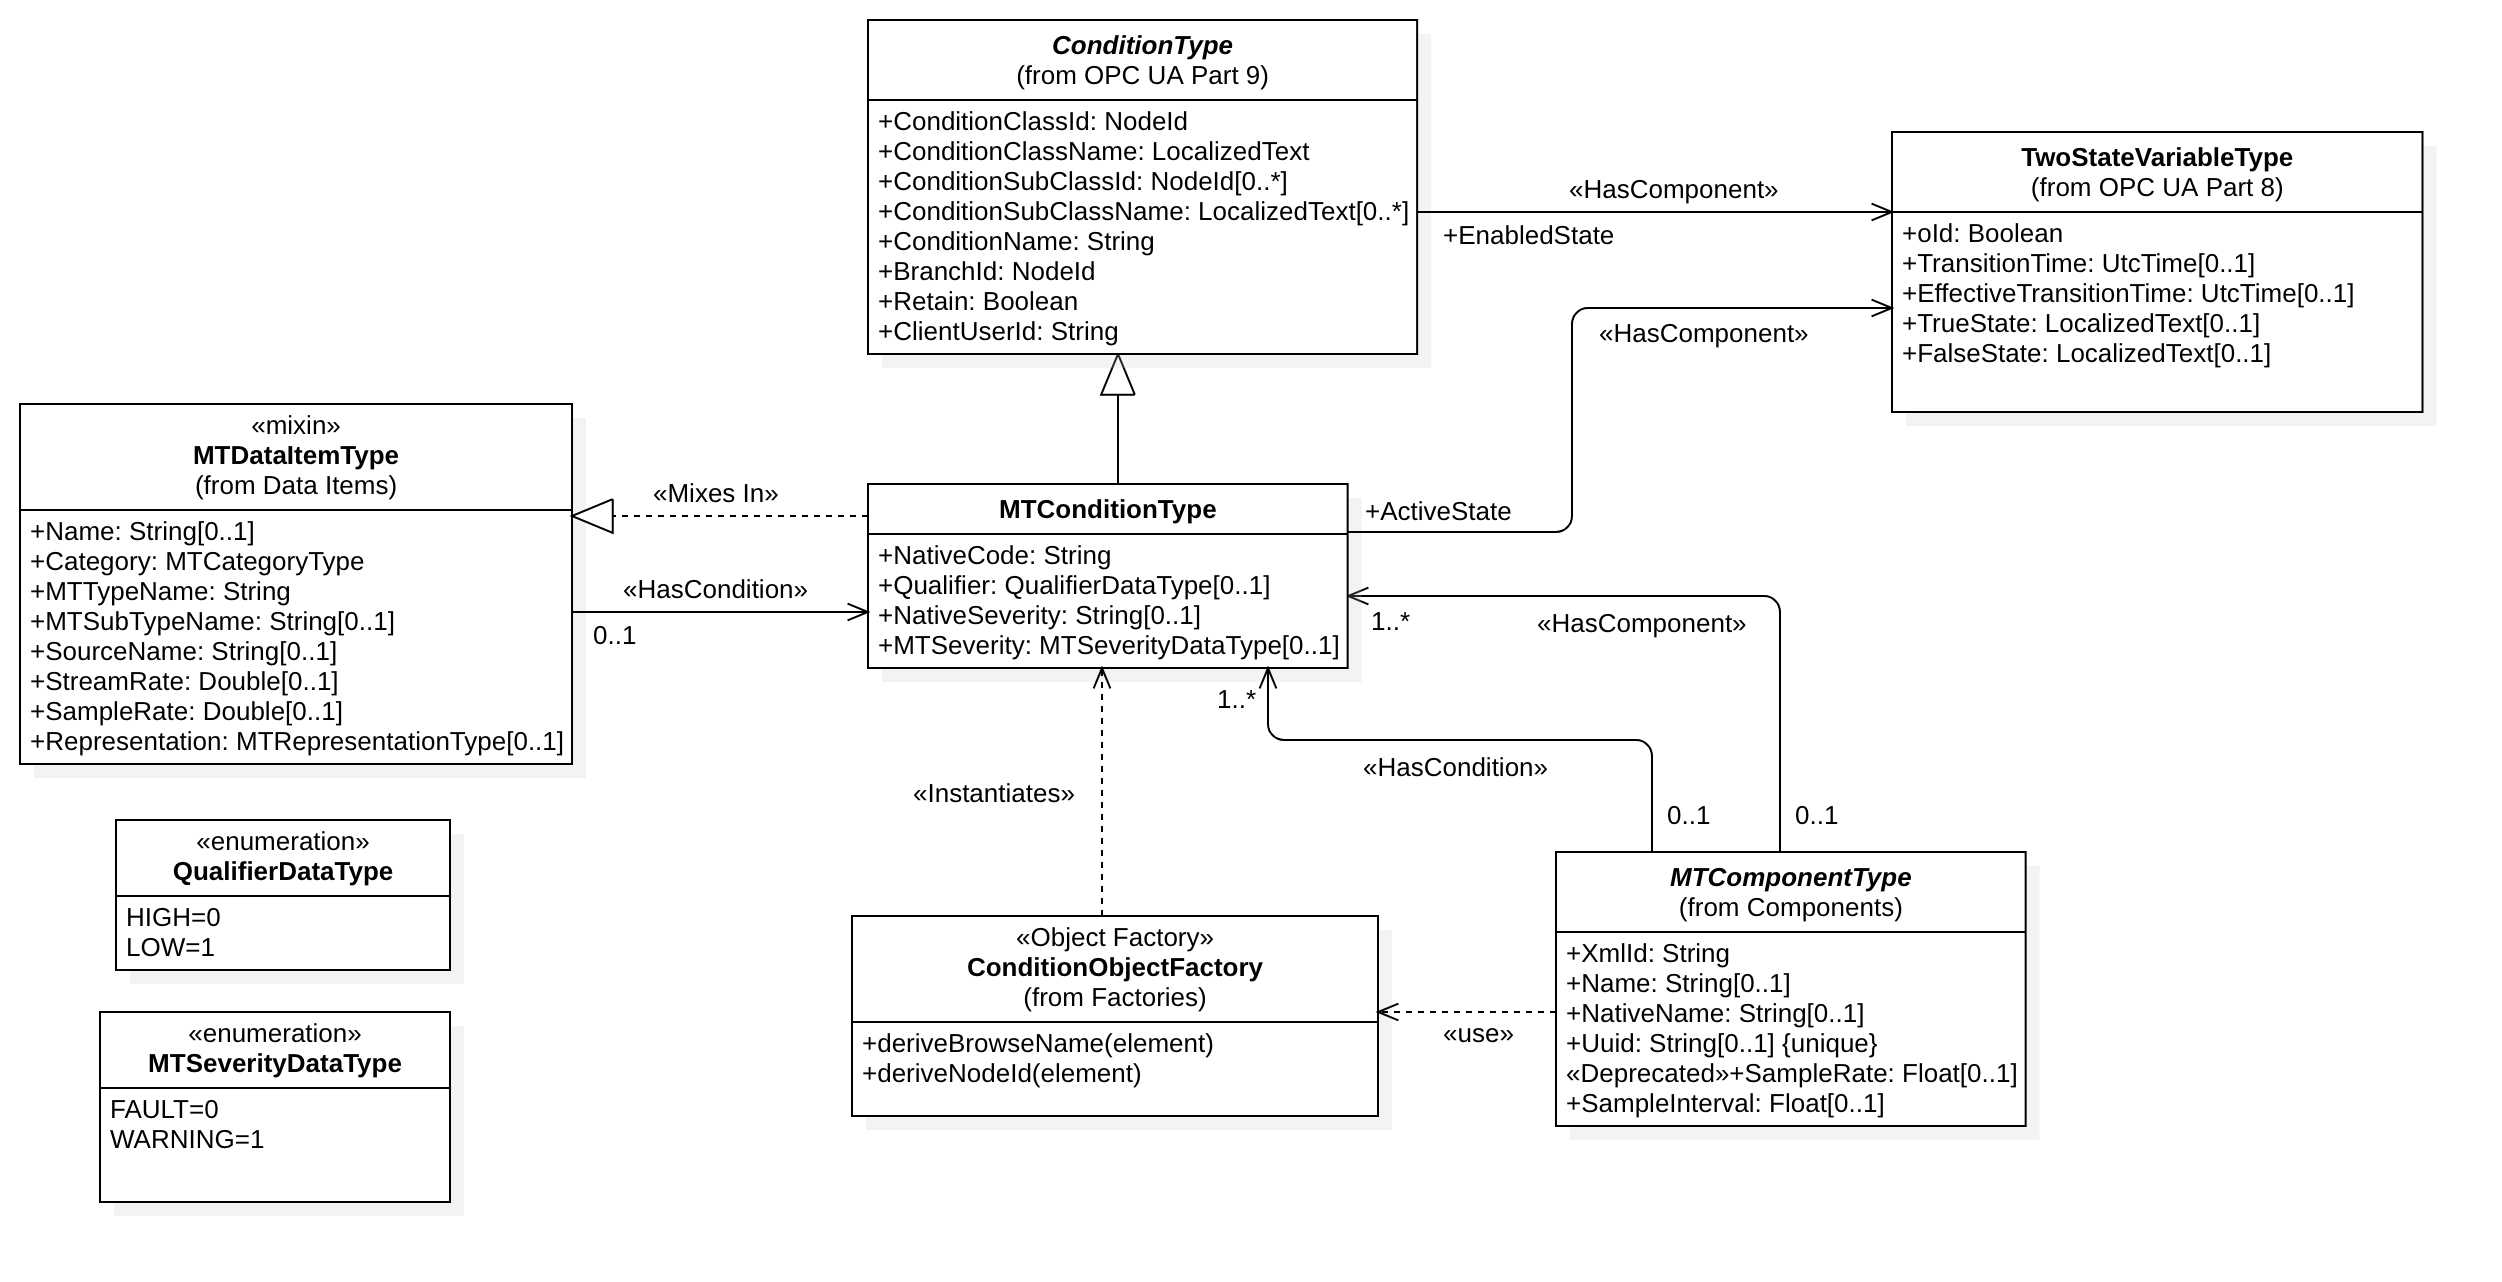
\includegraphics[width=1.0\textwidth]{diagrams/Conditions.png}
  \caption{Conditions Diagram}
  \label{fig:Conditions}
\end{figure}

\FloatBarrier




\subsubsection{Defintion of \texttt{ MTExclusiveLimitConditionType}} \label{type:MTExclusiveLimitConditionType}

\FloatBarrier



\begin{table}[ht]
\centering 
  \caption{\texttt{MTExclusiveLimitConditionType} Definition}
  \label{table:MTExclusiveLimitConditionType}
\fontsize{9pt}{11pt}\selectfont
\tabulinesep=3pt
\begin{tabu} to 6in {|l|l|l|l|l|l|} \everyrow{\hline}
\hline
\rowfont\bfseries {Attribute} & \multicolumn{5}{|l|}{Value} \\
\tabucline[1.5pt]{}
BrowseName & \multicolumn{5}{|l|}{MTExclusiveLimitConditionType} \\
IsAbstract & \multicolumn{5}{|l|}{False} \\
\tabucline[1.5pt]{}
\rowfont \bfseries References & NodeClass & BrowseName & DataType & TypeDefinition & {Modeling Rule} \\
\multicolumn{6}{|l|}{Subtype of ExclusiveLimitAlarmType (See OPCUA Documentation)} \\
\end{tabu}
\end{table} 


\paragraph{Dependency on MTDataItemType}

This class relates to \texttt{MTDataItemType} (See section \ref{type:MTDataItemType}) for a(n) \texttt{Mixes  In} relationship.

\FloatBarrier
\subsubsection{Defintion of \texttt{ MTNonExclusiveConditionType}} \label{type:MTNonExclusiveConditionType}

\FloatBarrier



\begin{table}[ht]
\centering 
  \caption{\texttt{MTNonExclusiveConditionType} Definition}
  \label{table:MTNonExclusiveConditionType}
\fontsize{9pt}{11pt}\selectfont
\tabulinesep=3pt
\begin{tabu} to 6in {|l|l|l|l|l|l|} \everyrow{\hline}
\hline
\rowfont\bfseries {Attribute} & \multicolumn{5}{|l|}{Value} \\
\tabucline[1.5pt]{}
BrowseName & \multicolumn{5}{|l|}{MTNonExclusiveConditionType} \\
IsAbstract & \multicolumn{5}{|l|}{False} \\
\tabucline[1.5pt]{}
\rowfont \bfseries References & NodeClass & BrowseName & DataType & TypeDefinition & {Modeling Rule} \\
\multicolumn{6}{|l|}{Subtype of NonEclusiveLimitAlarmType (See OPCUA Documentation)} \\
\end{tabu}
\end{table} 


\paragraph{Dependency on MTDataItemType}

This class relates to \texttt{MTDataItemType} (See section \ref{type:MTDataItemType}) for a(n) \texttt{Mixes  In} relationship.

\FloatBarrier
\subsubsection{Defintion of \texttt{<<Dynamic Type>> \{ConditionClass\}Type}} \label{type:{ConditionClass}Type}

\FloatBarrier



\begin{table}[ht]
\centering 
  \caption{\texttt{\{ConditionClass\}Type} Definition}
  \label{table:{ConditionClass}Type}
\fontsize{9pt}{11pt}\selectfont
\tabulinesep=3pt
\begin{tabu} to 6in {|l|l|l|l|l|l|} \everyrow{\hline}
\hline
\rowfont\bfseries {Attribute} & \multicolumn{5}{|l|}{Value} \\
\tabucline[1.5pt]{}
BrowseName & \multicolumn{5}{|l|}{{ConditionClass}Type} \\
IsAbstract & \multicolumn{5}{|l|}{False} \\
\tabucline[1.5pt]{}
\rowfont \bfseries References & NodeClass & BrowseName & DataType & TypeDefinition & {Modeling Rule} \\
\multicolumn{6}{|l|}{Subtype of SystemConditionClassType (See OPCUA Documentation)} \\
\end{tabu}
\end{table} 


\FloatBarrier
\subsection{Factories}

\begin{figure}[ht]
  \centering
    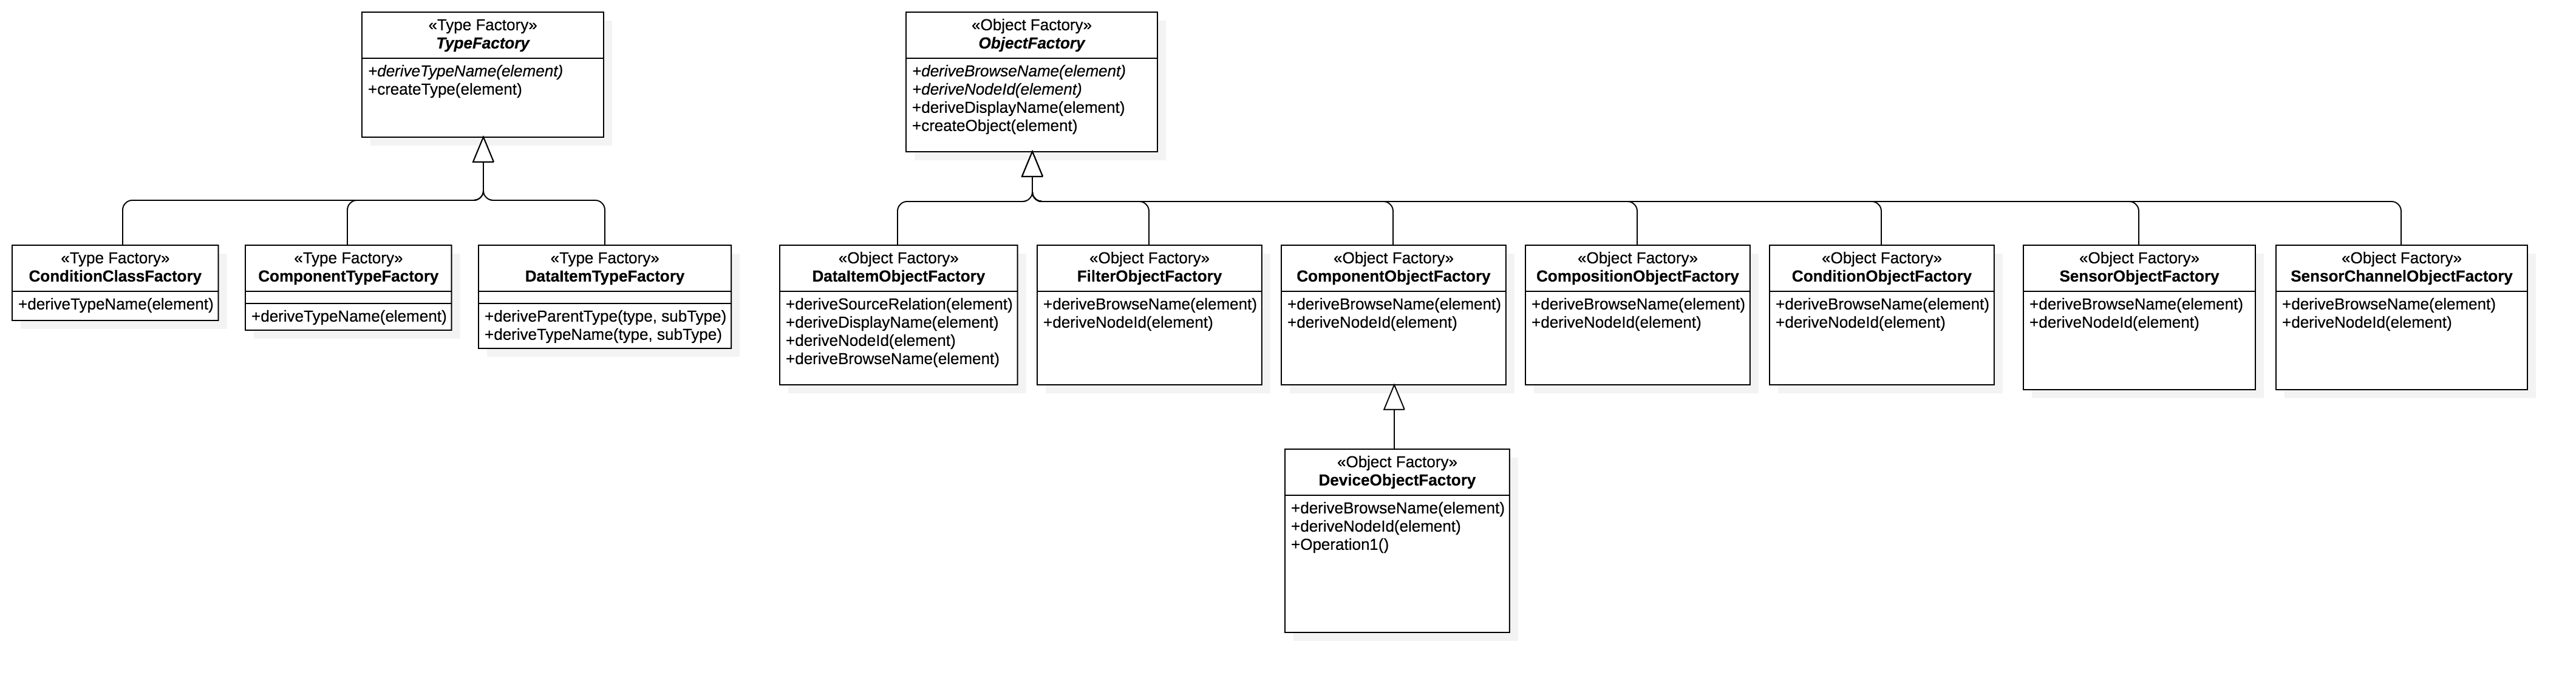
\includegraphics[width=1.0\textwidth]{diagrams/Factories.png}
  \caption{Factories Diagram}
  \label{fig:Factories}
\end{figure}

\FloatBarrier


The factories are not part of the OPC/UA information model. They are a set of helper 
classes that are used to create dynamic types and objects. Since the MTConnect 
information model can be layered on top of the OPC/UA abstrations, the factories
provide the rules for creating the browse and display names for each type.

The factories also create dynamic objects when requried for variables of various
classes when they are required, such as the Data Items and the Components. Some of the
relationships are more complex since they require a dynamic super-type relationship that
relies on the correct placement of the MTConnect elements to be correctly 
represented using the OPC/UA base types.

This is especially evident when mapping the DataItems and the Conditions to the 
MTConnect Information Models and providing sufficent definition to allow for 
unambiguous implementation.

\subsubsection{Defintion of \texttt{<<Object Factory>> ComponentObjectFactory}} \label{type:ComponentObjectFactory}

\FloatBarrier



\paragraph{Operations}
\begin{itemize}
  \item \texttt{deriveBrowseName(element)}\\
    Specification:
   \indent \begin{Verbatim}[xleftmargin=.25in,fontsize=\small]
concat(element.QName, (if self.name.notEmpty() then concat('[', self.name, ']')) else  '' endif))
\end{Verbatim}

  \item \texttt{deriveNodeId(element)}\\
    Specification:
   \indent \begin{Verbatim}[xleftmargin=.25in,fontsize=\small]
concat(self.findDevice().uuid, element.id)
\end{Verbatim}

\end{itemize}
\FloatBarrier
\subsubsection{Defintion of \texttt{<<Type Factory>> ComponentTypeFactory}} \label{type:ComponentTypeFactory}

\FloatBarrier

The `ComponentTypeFactory` creates component types using the MTConnect XML element as an input. 
The factory takes the `QName` (or qualified name) of the XML element and then appends `Type`. For 
example an `<Controller id='...'></...>` element will create an OPC/UA `ControllerType` type definition 
as an extension of the base `MTControllerType`. 

Currently there is no additional abstractions or super types required by the companion specification. 
The types will be a single level where each Component is a sub-type of the base `MTComponentType`.


\paragraph{Operations}
\begin{itemize}
  \item \texttt{deriveTypeName(element)}\\
    Specification:
   \indent \begin{Verbatim}[xleftmargin=.25in,fontsize=\small]
derive: Component <- element.QName
\end{Verbatim}

    Documentation: The QName of the element for the component will be used to derive the type of the node.

\end{itemize}
\paragraph{Dependency on {Component}Type}

This class relates to \texttt{{Component}Type} (See section \ref{type:{Component}Type}) for a(n) \texttt{Instantiates} relationship.

\FloatBarrier
\subsubsection{Defintion of \texttt{<<Object Factory>> CompositionObjectFactory}} \label{type:CompositionObjectFactory}

\FloatBarrier



\paragraph{Operations}
\begin{itemize}
  \item \texttt{deriveBrowseName(element)}\\
    Specification:
   \indent \begin{Verbatim}[xleftmargin=.25in,fontsize=\small]
concat(pascalCase(element.type), (if self.name.notEmpty() then concat('[', self.name, ']')) else  '' endif))
\end{Verbatim}

  \item \texttt{deriveNodeId(element)}\\
    Specification:
   \indent \begin{Verbatim}[xleftmargin=.25in,fontsize=\small]
concat(self.findDevice().uuid, element.id)
\end{Verbatim}

\end{itemize}
\paragraph{Dependency on {Composition}Type}

This class relates to \texttt{{Composition}Type} (See section \ref{type:{Composition}Type}) for a(n) \texttt{Instantiates} relationship.

\FloatBarrier
\subsubsection{Defintion of \texttt{<<Type Factory>> CompositionTypeFactory}} \label{type:CompositionTypeFactory}

\FloatBarrier



\paragraph{Operations}
\begin{itemize}
  \item \texttt{deriveTypeName(element)}\\
    Specification:
   \indent \begin{Verbatim}[xleftmargin=.25in,fontsize=\small]
derive: Composition <-
 pascalCase(element.type)
\end{Verbatim}

    Documentation: The type for the composition will be created using the pascal case of the `type` from the composition element.

\end{itemize}
\FloatBarrier
\subsubsection{Defintion of \texttt{<<Type Factory>> ConditionClassFactory}} \label{type:ConditionClassFactory}

\FloatBarrier



\paragraph{Operations}
\begin{itemize}
  \item \texttt{deriveTypeName(element)}
    Documentation: Create condition classes based on the OPC/UA three condition  types.

\end{itemize}
\FloatBarrier
\subsubsection{Defintion of \texttt{<<Object Factory>> ConditionObjectFactory}} \label{type:ConditionObjectFactory}

\FloatBarrier



\paragraph{Operations}
\begin{itemize}
  \item \texttt{deriveBrowseName(element)}
  \item \texttt{deriveNodeId(element)}
\end{itemize}
\paragraph{Dependency on MTExclusiveLimitConditionType}

This class relates to \texttt{MTExclusiveLimitConditionType} (See section \ref{type:MTExclusiveLimitConditionType}) for a(n) \texttt{Instantiates} relationship.

\paragraph{Dependency on MTNonExclusiveConditionType}

This class relates to \texttt{MTNonExclusiveConditionType} (See section \ref{type:MTNonExclusiveConditionType}) for a(n) \texttt{Instantiates} relationship.

\FloatBarrier
\subsubsection{Defintion of \texttt{<<Object Factory>> DataItemObjectFactory}} \label{type:DataItemObjectFactory}

\FloatBarrier



\paragraph{Operations}
\begin{itemize}
  \item \texttt{deriveSourceRelation(element)}
    Documentation: Use the source composition,  component id, or data item id to locate the source node id for this relationship. If one exists, add an object with  browse name "source" that relates to the entity referenced by the id. 

The most specific identity should be used in the following order:
\begin{itemize}
\item \texttt{DataItemId}
\item \texttt{CompositionId}
\item \texttt{ComponentId}
\end{itemize}

Since the data item implies composition and component and the composition implies component, there should only be one attribute given for the source.

  \item \texttt{deriveDisplayName(element)}
    Documentation: Same as the BrowseName.

  \item \texttt{deriveNodeId(element)}
    Documentation: The nodeId will be given by the device uuid and the DataItem id attribute.

  \item \texttt{deriveBrowseName(element)}
    Documentation: The browse name will be composed of the following parts of the model:

\begin{enumerate}
\item If the compositionId is present, the compositionId will be resolved the the Composition element and the pascal case of the type attribute will be placed first.
\item If the subType is present, the pascal case of the subType will be placed next.
\item The pascal case of the type will be placed last.
\end{enumerate}

For example, for a data item with the following attributes:

\begin{itemize}
\item type: \texttt{TEMPERATURE}
\item composition type: \texttt{STORAGE_BATTERY}
\end{itemize}

will have the following browse name: \texttt{StorageBatteryTemperature}

For the data item with the following attributes:

\begin{itemize}
\item type: \texttt{ANGLE}
\item subType: \texttt{ACTUAL}
\item composition type: \texttt{ENCODER}
\end{itemize}

will have the following browse name: \texttt{EncoderActualAngle}


\end{itemize}
\paragraph{Dependency on MTMessageType}

This class relates to \texttt{MTMessageType} (See section \ref{type:MTMessageType}) for a(n) \texttt{Instantiates} relationship.

\paragraph{Dependency on AssetChangedType}

This class relates to \texttt{AssetChangedType} (See section \ref{type:AssetChangedType}) for a(n) \texttt{Instantiates} relationship.

\paragraph{Dependency on AssetRemovedType}

This class relates to \texttt{AssetRemovedType} (See section \ref{type:AssetRemovedType}) for a(n) \texttt{Instantiates} relationship.

\FloatBarrier
\subsubsection{Defintion of \texttt{<<Type Factory>> DataItemTypeFactory}} \label{type:DataItemTypeFactory}

\FloatBarrier

Based on the data item category, type, and subType, this class creates a new OPC/UA type 
and also provides the template parameter for the ParentType from which this type is derived. 


\paragraph{Operations}
\begin{itemize}
  \item \texttt{deriveParentType(type, subType)}
    Documentation: The parent type is derived from the category as follows: 

\begin{itemize}
  \item \texttt{SAMPLE} -> \texttt{SampleType}
  \item \texttt{EVENT} ->
  \begin{itemize}
   \item Enumerated Value -> \texttt{MTEnumeratedEventType}
   \item Integer Value -> \texttt{MTNumericEventType}
   \item Otherwise -> \texttt{MTStringEventType}
  \end{itemize}
\end{itemize}

  \item \texttt{deriveTypeName(type, subType)}\\
    Specification:
   \indent \begin{Verbatim}[xleftmargin=.25in,fontsize=\small]
concat(pascalCase(subType), pascalCase(type))
\end{Verbatim}

    Documentation: Used to derive the class name for creating a pascal case name from the sub type and the type. 
For example type \texttt{ROTARY_VELOCITY} and subType \texttt{ACTUAL} will become \texttt{ActualRotaryVelocity}.

\end{itemize}
\paragraph{Dependency on {DataItem}Type}

This class relates to \texttt{{DataItem}Type} (See section \ref{type:{DataItem}Type}) for a(n) \texttt{Instantiates} relationship.

\FloatBarrier
\subsubsection{Defintion of \texttt{<<Object Factory>> DeviceObjectFactory}} \label{type:DeviceObjectFactory}

\FloatBarrier

The model instantiation for MTConnect begins with the `Device` MTConnect element and then recursively traverses the sub-elements. The device will the capabilities in the component factory to generate all the data items and component types. 

\paragraph{Operations}
\begin{itemize}
  \item \texttt{deriveBrowseName(element)}\\
    Specification:
   \indent \begin{Verbatim}[xleftmargin=.25in,fontsize=\small]
derive: element.name
\end{Verbatim}

  \item \texttt{deriveNodeId(element)}\\
    Specification:
   \indent \begin{Verbatim}[xleftmargin=.25in,fontsize=\small]
derive: element.uuid
\end{Verbatim}

\end{itemize}
\paragraph{Dependency on MTDeviceType}

This class relates to \texttt{MTDeviceType} (See section \ref{type:MTDeviceType}) for a(n) \texttt{Instantiates} relationship.

\FloatBarrier
\subsubsection{Defintion of \texttt{<<Object Factory>> FilterObjectFactory}} \label{type:FilterObjectFactory}

\FloatBarrier

Creates filters based on the type attribute of the Filter element. 

\paragraph{Operations}
\begin{itemize}
  \item \texttt{deriveBrowseName(element)}
  \item \texttt{deriveNodeId(element)}
    Documentation: The node id is composed of the data item id and the browse name.

\end{itemize}
\paragraph{Dependency on MinimumDeltaFilterType}

This class relates to \texttt{MinimumDeltaFilterType} (See section \ref{type:MinimumDeltaFilterType}) for a(n) \texttt{Instantiates} relationship.

\paragraph{Dependency on PeriodFilterType}

This class relates to \texttt{PeriodFilterType} (See section \ref{type:PeriodFilterType}) for a(n) \texttt{Instantiates} relationship.

\FloatBarrier
\subsubsection{Defintion of \texttt{<<Object Factory>> ObjectFactory}} \label{type:ObjectFactory}

\FloatBarrier



\paragraph{Operations}
\begin{itemize}
  \item \texttt{deriveBrowseName(element)}
  \item \texttt{deriveNodeId(element)}
  \item \texttt{deriveDisplayName(element)}\\
    Specification:
   \indent \begin{Verbatim}[xleftmargin=.25in,fontsize=\small]
deriveBrowseName(element)
\end{Verbatim}

  \item \texttt{createObject(element)}
\end{itemize}
\FloatBarrier
\subsubsection{Defintion of \texttt{<<Object Factory>> SensorChannelObjectFactory}} \label{type:SensorChannelObjectFactory}

\FloatBarrier



\paragraph{Operations}
\begin{itemize}
  \item \texttt{deriveBrowseName(element)}\\
    Specification:
   \indent \begin{Verbatim}[xleftmargin=.25in,fontsize=\small]
concat('Channel', self.number)
\end{Verbatim}

  \item \texttt{deriveNodeId(element)}\\
    Specification:
   \indent \begin{Verbatim}[xleftmargin=.25in,fontsize=\small]
concat(self.parent.NodeId, BrowseName)
\end{Verbatim}

\end{itemize}
\paragraph{Dependency on ChannelType}

This class relates to \texttt{ChannelType} (See section \ref{type:ChannelType}) for a(n) \texttt{Instantiates} relationship.

\FloatBarrier
\subsubsection{Defintion of \texttt{<<Object Factory>> SensorObjectFactory}} \label{type:SensorObjectFactory}

\FloatBarrier



\paragraph{Operations}
\begin{itemize}
  \item \texttt{deriveBrowseName(element)}\\
    Specification:
   \indent \begin{Verbatim}[xleftmargin=.25in,fontsize=\small]
element.QName
\end{Verbatim}

  \item \texttt{deriveNodeId(element)}\\
    Specification:
   \indent \begin{Verbatim}[xleftmargin=.25in,fontsize=\small]
concat(self.parent.NodeId, BrowseName)
\end{Verbatim}

\end{itemize}
\paragraph{Dependency on SensorConfigurationType}

This class relates to \texttt{SensorConfigurationType} (See section \ref{type:SensorConfigurationType}) for a(n) \texttt{Instantiates} relationship.

\FloatBarrier
\subsubsection{Defintion of \texttt{<<Type Factory>> TypeFactory}} \label{type:TypeFactory}

\FloatBarrier



\paragraph{Operations}
\begin{itemize}
  \item \texttt{deriveTypeName(element)}
  \item \texttt{createType(element)}
\end{itemize}
\FloatBarrier
\subsection{MTConnect Device Profile}

\begin{figure}[ht]
  \centering
    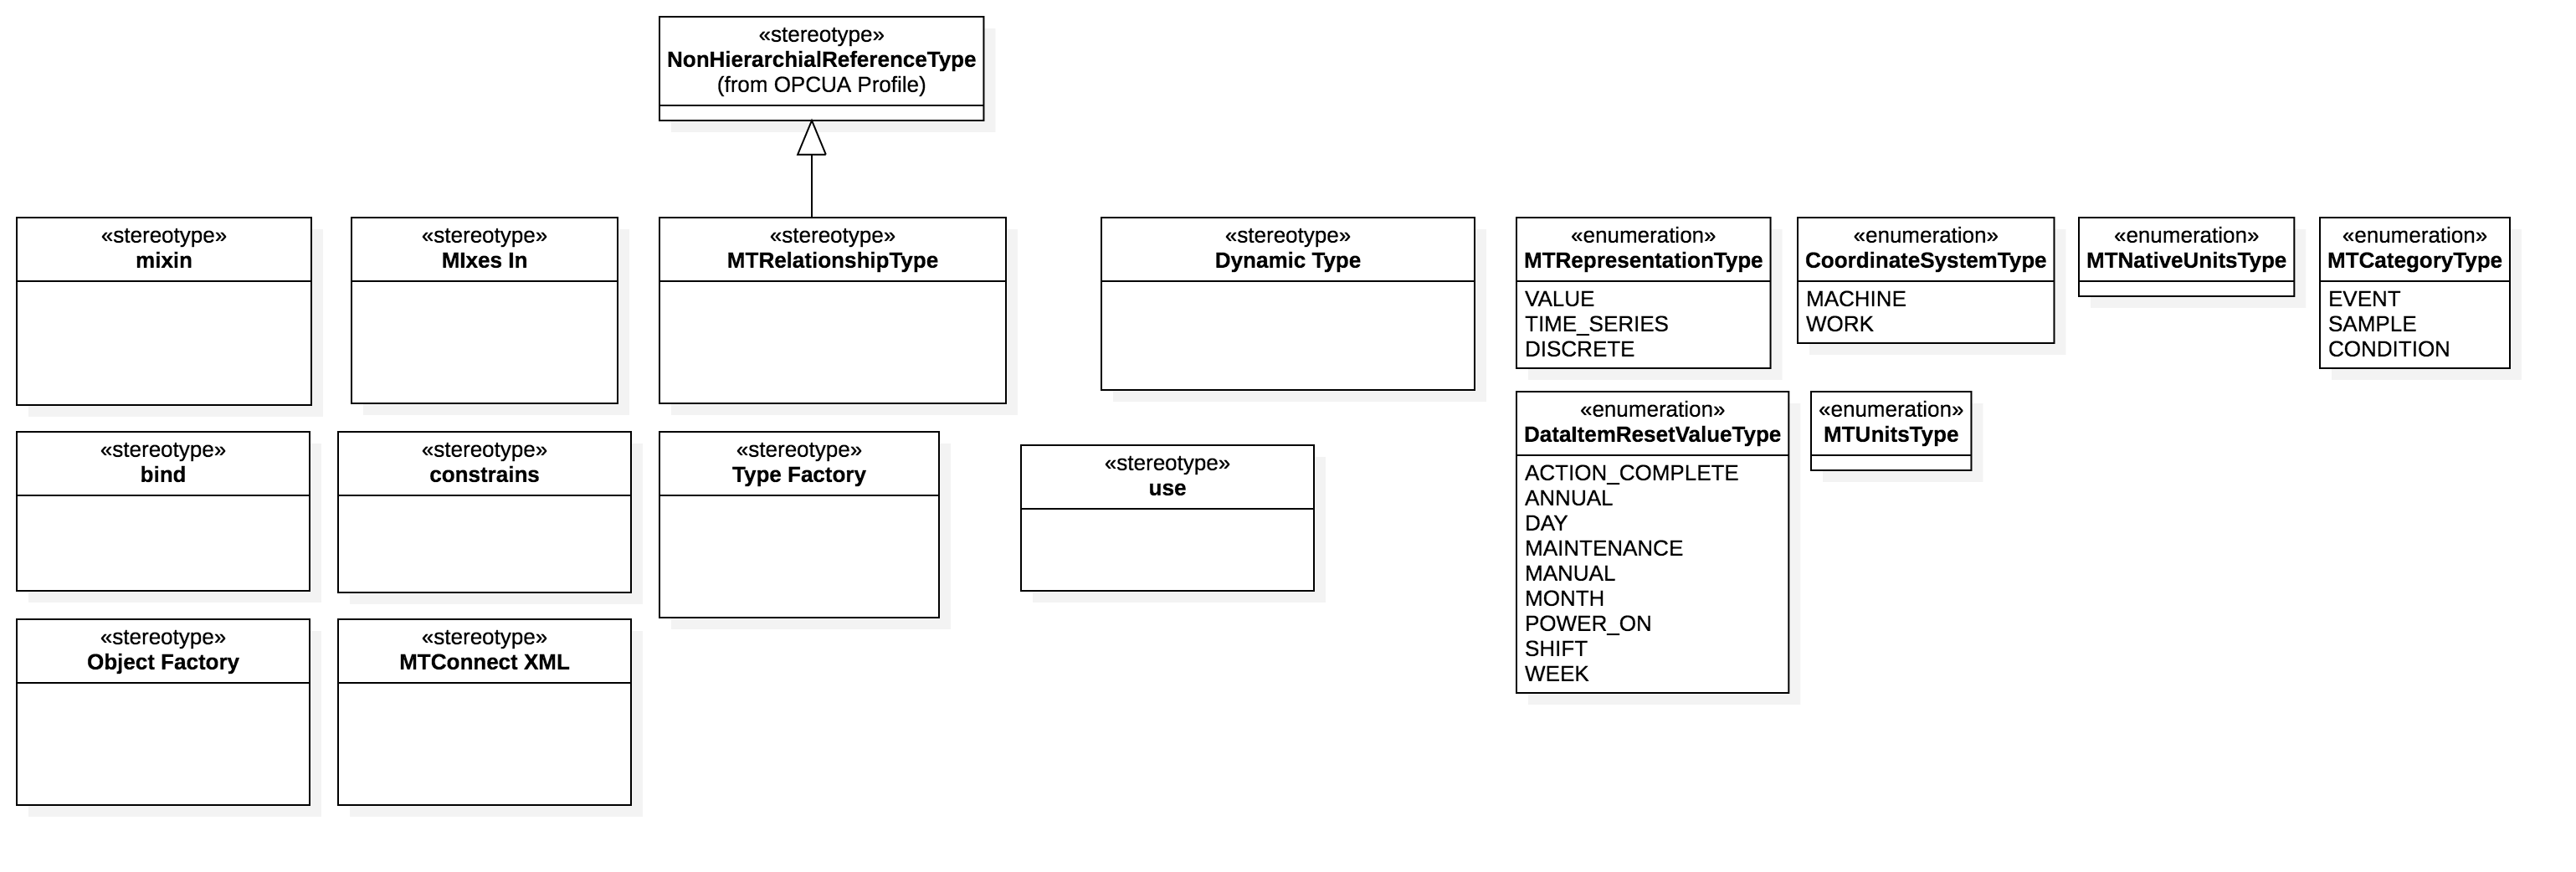
\includegraphics[width=1.0\textwidth]{diagrams/MTConnect Device Profile.png}
  \caption{MTConnect Device Profile Diagram}
  \label{fig:MTConnect Device Profile}
\end{figure}

\FloatBarrier


The device profile documents the common data types and stereotypes that are 
used to construct the model. A stereotype is a design or modeling pattern that 
provides additional information about the type or the relationship between types. 

It can also identify the behavior of a property or the role the type or relation
will play in the model. 

Stereotypes are used throughout the model to provide additional information that 
will halp provide context and definition to aid in better understanding the
data model.

\subsubsection{Defintion of \texttt{ Dynamic Type}} \label{type:Dynamic Type}

\FloatBarrier



\FloatBarrier
\subsubsection{Defintion of \texttt{ MTConnect XML}} \label{type:MTConnect XML}

\FloatBarrier



\FloatBarrier
\subsubsection{Defintion of \texttt{ MTRelationshipType}} \label{type:MTRelationshipType}

\FloatBarrier



\FloatBarrier
\subsubsection{Defintion of \texttt{ Mixes  In}} \label{type:Mixes  In}

\FloatBarrier

This stereotype is associated with the dependency between a type and a mixin. See Section \ref{type:mixin} for a complete 
description of the mixin.

\FloatBarrier
\subsubsection{Defintion of \texttt{ Object Factory}} \label{type:Object Factory}

\FloatBarrier



\FloatBarrier
\subsubsection{Defintion of \texttt{<<Type Factory>> Type Factory}} \label{type:Type Factory}

\FloatBarrier



\FloatBarrier
\subsubsection{Defintion of \texttt{ bind}} \label{type:bind}

\FloatBarrier

When a dynamic type (See Section \ref{type:Dynamic Type}) creates an instance where the super-type
can be associated based on the data item category and type, the \texttt{Type Factory} will 
specify which supertype is to be referenced.

The \texttt{bind} stereotype indicates the relationship between the dynamic sub-type and the 
parent type are resolved baed on the MTConnect DataItem meta data.

\FloatBarrier
\subsubsection{Defintion of \texttt{ constrains}} \label{type:constrains}

\FloatBarrier



\FloatBarrier
\subsubsection{Defintion of \texttt{ mixin}} \label{type:mixin}

\FloatBarrier

The mixin pattern injects the properties and operations into the types 
that are related to the using the \texttt{Mixes In} dependency. Mixins allow for
lightweight multiple inheritance. Since OPC/UA does not allow for multiple inheritance 
and the MTConnect  types require the same set of properties when they are sub-typed
from existing OPC/UA types, this mechanism allows for this relationship to be expressed.


\FloatBarrier
\subsubsection{Defintion of \texttt{ use}} \label{type:use}

\FloatBarrier

The use stereotype indicates that one class uses as a helper to perform 
a specific operation or activity. This stereotype is mainly used to indicate
that a specific factory is being employed by another type to create dynamic
properties or relationships.

\FloatBarrier
\subsubsection{Defintion of \texttt{ values}} \label{type:values}

\FloatBarrier

For controlled vocabularies of enumerated types, specifies the relationship to the allowable 
values for the type.

\FloatBarrier
